 % % Preamble BEGINN %%%%%%%%%%%%%%%%%%%%%%%%%%%%%%%%%%%%%%%%%%%%%%%%%%%%%%%%%

%%% Preamble (Dokumentenklasse)
% ------------------------------------------------------------------------
% LaTeX - Preambel ******************************************************
% ------------------------------------------------------------------------
% Dokumentklasse (Koma Script)
% ------------------------------------------------------------------------
% basiernd auf www.matthiaspospiech.de/latex/vorlagen Diplomarbeit kompakt
% ========================================================================
\documentclass[%
   %draft,            % Entwurfsstadium
   final,             % fertiges Dokument
   12pt,              % Schriftgroesse der Grundschrift
   bigheadings,       % gro�e �berschriften
   ngerman,           % wird an andere Pakete weitergereicht
   a4paper,           % Papierformat
   BCOR5mm,          % Bindekorrektur: Zus�tzlicher Rand auf der Innenseite
   DIV14,            % Seitengr��e (siehe Koma Skript Dokumentation !)
   1.1headlines,     % Zeilenanzahl der Kopfzeilen
   pagesize,         % Schreibt die Papiergroesse in die Datei.
   oneside,          % Einseitiges Layout
%   twoside,          % Zweiseitiges Layout
   openright,        % Kapitel beginnen immer auf der rechten Seite
   titlepage,        % Titel als einzelne Seite ('titlepage' Umgebung)  
   headsepline,      % Linie unter Kolumnentitel ()
%   plainheadsepline, % Linie unter Kolumnentitel () plain Seitenstil
   nochapterprefix,  % keine Ausgabe von 'Kapitel:'
   bibtotoc,         % Bibliographie ins TOC
%	bibtotocnumbered, % Bibliographie ins TOC mit Kapitelnummer
   tocindent,        % eingereuckte Gliederung
   listsindent,      % eingereuckte LOT, LOF
   pointlessnumbers, % �berschriftnummerierung ohne Punkt, siehe DUDEN !
   cleardoubleempty, % Leere linke Seite bei Zweiseitenlayout vor Kapitel
   fleqn,            % Formeln werden linksbuendig angezeigt
%   parindent,        % Absatz mit Einzug (Standard)
   halfparskip,      % Absatz halbe Zeile Abstand
%   parskip,          % Absatz ganze Zeile Abstand
]{scrbook}%     Klassen: scrartcl, scrreprt, scrbook


%%% Alle Namen usw. im Titel und im hyperref-Paket
% ------------------------------------------------------------------------
% LaTeX - Preambel ******************************************************
% ------------------------------------------------------------------------
% pre-work
% ========================================================================
% % ToDo kennzeichnen
\newcommand{\workTodo}[1]{\textcolor{red}{todo: #1}}

% % F�r Datum und Zeit in Fusszeile
% % !!!Inhalt bei Fertigstellung der Arbeit l�schen
\newcommand{\workMarkDateTime}{\today}

% % Alle Namen werden im Titel und im hyperref-Paket eingetragen
% % !!! Ueberall f�r <Wert> das Entsprechende eintragen

 % <Typ> Studienarbeit, Dipolmarbeit, Studienarbeit oder Bachlor-Abschlussarbeit
\newcommand{\workTyp}{Masterquad 2015\xspace}

 % <Titel> der Arbeit
\newcommand{\workTitel}{A Raspberry Pi based quadrocopter platform}

 % <Studiengang> z.B. Kommunikationstechnik
\newcommand{\workStudiengang}{Software-based Automotive Systems (ASM-SB) \xspace}

% <Semester> mit Jahr z.B. Sommersemester 2008  
\newcommand{\workSemester}{Summer term 2015\xspace}

% <Name> des Studenten
\newcommand{\workNameStudentOne}{Oliver Breuning\xspace}
\newcommand{\workNameStudentTwo}{J\"urgen Schmidt\xspace}
\newcommand{\workNameStudentThree}{Martin Brodbeck\xspace}
\newcommand{\workNameStudentFour}{Phillip Woditsch\xspace}
\newcommand{\workNameStudentFive}{Chris M\"onch\xspace}


% <Pruefer> Name des pr�fenden (betreuenden) Professor an der Hochschule
\newcommand{\workPruefer}{\\Prof. Dr. J\"org Friedrich\\M Sc. Vikas Agrawal\xspace} 
%\newcommand{\workPruefer}{M Sc. Vikas Agrawal\xspace} 


% %%% Nur bei Abschluss-Arbeiten

% <Datum> der Abgabe der Arbeit (Eidesstatliche Erkl�rung)
\newcommand{\workDatum}{\today\xspace}

% <Zweitpr�fer>
\newcommand{\workZweitPruefer}{\workTodo{<Zweitpr�fer>}\xspace}

% <Zeitraum>
\newcommand{\workZeitraum}{Summer term 2015\xspace}


% %%% Nur bei Industrie-Arbeiten:

% <Firma>
\newcommand{\workFirma}{\workTodo{<Firma>}\xspace}

% <Betreuer in der Firma>
\newcommand{\workBetreuer}{\workTodo{<Betreuer in der Firma>}\xspace}

% Firmenlogo Name hier anpassen, Gr��e (wenn m�glich) nicht �ndern
%\newcommand{\workFirmenLogo}{
\includegraphics[width=5cm]{fig/aa-titel/Bosch_4C_S}} 


%%% Preamble (Pakete)
% ------------------------------------------------------------------------
% LaTeX - Preambel ******************************************************
% ------------------------------------------------------------------------
% Packages
% ------------------------------------------------------------------------
% basiernd auf www.matthiaspospiech.de/latex/vorlagen Diplomarbeit kompakt
% ========================================================================

% Inhalt:
% 1. Einige Pakete muessen unbedingt vor allen anderen geladen werden
% 2. Fonts Fonts Fonts
% 3. Math Packages
% 4. Symbole
% 5. text related packages
% 6. Pakete zum Zitieren
% 7. PDF related packages
% 8. Tables (Tabular)
% 9. figures and placement
% 10. verbatim packages
% 11. science packages
% 12. layout packages

% ~~~~~~~~~~~~~~~~~~~~~~~~~~~~~~~~~~~~~~~~~~~~~~~~~~~~~~~~~~~~~~~~~~~~~~~~
% Encoding der Dateien (sonst funktionieren Umlaute nicht)
% Empfohlen latin1, da einige Pakete mit utf8 Zeichen nicht
% funktionieren, z.B: listings, soul.

\usepackage[latin1]{inputenx} % ISO-8859-1
%\usepackage[ansinew]{inputenx} % Windows-Standard (CP1252) (baut auf ISO 8859-1 und ISO 8859-15 auf)
%\usepackage[utf8]{inputenc}

% ~~~~~~~~~~~~~~~~~~~~~~~~~~~~~~~~~~~~~~~~~~~~~~~~~~~~~~~~~~~~~~~~~~~~~~~~
% 1. Einige Pakete muessen unbedingt vor allen anderen geladen werden
% ~~~~~~~~~~~~~~~~~~~~~~~~~~~~~~~~~~~~~~~~~~~~~~~~~~~~~~~~~~~~~~~~~~~~~~~~
%
\usepackage{xspace} % Define commands that don't eat spaces.
\usepackage{ifpdf} % Fuer Pakete/Paketoptionen, die nur fuer pdf benoetigt werden \ifpdf \else \fi
\usepackage{calc} % Calculation with LaTeX
\usepackage[english]{babel} % Languagesetting
\usepackage[]{xcolor} % Farben
\usepackage{colortbl}
\usepackage[]{graphicx} % Bilder
%\usepackage{epstopdf} % If an eps image is detected, epstopdf is automatically called to convert it to pdf format.
\usepackage[]{amsmath} % Amsmath - Mathematik Basispaket
\usepackage{ragged2e} % Besserer Flatternsatz (Linksbuendig, statt Blocksatz)
\usepackage{hhline}
\usepackage{vhistory}
% ~~~~~~~~~~~~~~~~~~~~~~~~~~~~~~~~~~~~~~~~~~~~~~~~~~~~~~~~~~~~~~~~~~~~~~~~
% 2. Fonts Fonts Fonts
% ~~~~~~~~~~~~~~~~~~~~~~~~~~~~~~~~~~~~~~~~~~~~~~~~~~~~~~~~~~~~~~~~~~~~~~~~

\usepackage[T1]{fontenc} % T1 Schrift Encoding (notwendig f�r die meisten Type 1 Schriften)
\usepackage{textcomp}	 % Zusatzliche Symbole (Text Companion font extension)

% Alle Schriften die hier angegeben sind sehen im PDF richtig aus.
% Die LaTeX Standardschrift ist die Latin Modern (lmodern Paket).
% If Latin Modern is not available for your distribution you must install the
% package cm-super instead. Otherwise your fonts will look horrible in the PDF

% DO NOT LOAD ae-Package for the font !

%% - Latin Modern
\usepackage{lmodern}
%% -------------------
%
% % - Times, Helvetica, Courier (Word Standard...)
%\usepackage{mathptmx}
%\usepackage[scaled=.90]{helvet}
%\usepackage{courier}
% % -------------------
%%
%% - Palantino , Helvetica, Courier
%\usepackage{mathpazo}
%\usepackage[scaled=.95]{helvet}
%\usepackage{courier}
%% -------------------
%
%% - Bera Schriften
%\usepackage{bera}
%% -------------------
%
%% - Charter, Bera Sans
%\usepackage{charter}\linespread{1.05}
%\renewcommand{\sfdefault}{fvs}


% ~~~~~~~~~~~~~~~~~~~~~~~~~~~~~~~~~~~~~~~~~~~~~~~~~~~~~~~~~~~~~~~~~~~~~~~~
% 3. Math Packages
% ~~~~~~~~~~~~~~~~~~~~~~~~~~~~~~~~~~~~~~~~~~~~~~~~~~~~~~~~~~~~~~~~~~~~~~~~

\usepackage[fixamsmath,disallowspaces]{mathtools} % Erweitert amsmath und behebt einige Bugs
\usepackage{fixmath}
\usepackage[all,warning]{onlyamsmath} % Warnt bei Benutzung von Befehlen die mit amsmath inkompatibel sind.
\usepackage{icomma} % Erlaubt die Benutzung von Kommas im Mathematikmodus

% ~~~~~~~~~~~~~~~~~~~~~~~~~~~~~~~~~~~~~~~~~~~~~~~~~~~~~~~~~~~~~~~~~~~~~~~~
% 4. Symbole
% ~~~~~~~~~~~~~~~~~~~~~~~~~~~~~~~~~~~~~~~~~~~~~~~~~~~~~~~~~~~~~~~~~~~~~~~~
\usepackage{amssymb}
%\usepackage{wasysym}
%\usepackage{marvosym}
%\usepackage{pifont}

% ~~~~~~~~~~~~~~~~~~~~~~~~~~~~~~~~~~~~~~~~~~~~~~~~~~~~~~~~~~~~~~~~~~~~~~~~
% 5. text related packages
% ~~~~~~~~~~~~~~~~~~~~~~~~~~~~~~~~~~~~~~~~~~~~~~~~~~~~~~~~~~~~~~~~~~~~~~~~

\usepackage{url} % Setzen von URLs. In Verbindung mit hyperref sind diese auch aktive Links.
\usepackage[stable,perpage, ragged,  multiple]{footmisc} % Fussnoten
\usepackage[ngerman]{varioref} % Intelligente Querverweise
\usepackage{enumitem} % Listen

\usepackage{dirtree}


% ~~~~~~~~~~~~~~~~~~~~~~~~~~~~~~~~~~~~~~~~~~~~~~~~~~~~~~~~~~~~~~~~~~~~~~~~
% 6. Pakete zum Zitieren
% ~~~~~~~~~~~~~~~~~~~~~~~~~~~~~~~~~~~~~~~~~~~~~~~~~~~~~~~~~~~~~~~~~~~~~~~~

\usepackage[babel, german=quotes, english=british, french=guillemets]{csquotes} % clever quotations
\SetBlockThreshold{2} % Anzahl von Zeilen
\newenvironment{myquote}%
          {\begin{quote}\small}%
          {\end{quote}}%
\SetBlockEnvironment{myquote}

% ~~~~~~~~~~~~~~~~~~~~~~~~~~~~~~~~~~~~~~~~~~~~~~~~~~~~~~~~~~~~~~~~~~~~~~~~
% 7. PDF related packages
% ~~~~~~~~~~~~~~~~~~~~~~~~~~~~~~~~~~~~~~~~~~~~~~~~~~~~~~~~~~~~~~~~~~~~~~~~

\ifpdf % Wenn als PDF ausgegeben wird
\usepackage{pdfpages} % pdf-Seiten einbinden
\usepackage[pdftex]{hyperref} % PDF Option in Hyperref
\else
\usepackage[dvipdfm]{hyperref}
\fi

%%% Doc: ftp://tug.ctan.org/pub/tex-archive/macros/latex/contrib/pdfpages/pdfpages.pdf
%\usepackage{pdfpages} % Include pages from external PDF documents in LaTeX documents

%%% Doc: ftp://tug.ctan.org/pub/tex-archive/macros/latex/contrib/hyperref/doc/manual.pdf
\hypersetup{
          pdfhighlight = /O,	         % Visualisierung beim anklicken von Links
% Farben fuer die Links
   colorlinks=true,	        % Links erhalten Farben statt Kaestchen
   urlcolor=darkblue,    % \href{...}{...} external (URL)
   filecolor=darkblue,  % \href{...} local file
   linkcolor=darkblue,  % \ref{...} and \pageref{...}
          citecolor =darkblue,    % Literaturverzeichnis
   % Links
   raiselinks=true,			 % calculate real height of the link
   breaklinks,	        % Links bestehen bei Zeilenumbruch
%   backref=page,	         % Backlinks im Literaturverzeichnis (section, slide, page, none)
%   pagebackref=true,        % Backlinks im Literaturverzeichnis mit Seitenangabe
   verbose,
%   hyperindex=true,         % backlinkex index
   linktocpage=true,        % Inhaltsverzeichnis verlinkt Seiten
%   hyperfootnotes=false,	% Keine Links auf Fussnoten
   % Bookmarks
%   bookmarks=true,	         % Erzeugung von Bookmarks fuer PDF-Viewer
   bookmarksopenlevel=1,    % Gliederungstiefe der Bookmarks
   bookmarksopen=true,      % Expandierte Untermenues in Bookmarks
   bookmarksnumbered=true,  % Nummerierung der Bookmarks
   bookmarkstype=toc,       % Art der Verzeichnisses
   % Anchors
   plainpages=false,        % % Make page anchors using the formatted form of the page number. With this option, hyperref writes different anchors for pages �ii� and �2�. (If the option is set �true� � the default � hyperref writes page anchors as the arabic form of the absolute page number, rather than the formatted form.)
   % hypertexnames=false,
   pageanchor=true,	        % Pages are linkable
   % PDF Informationen
   pdftitle={\workTyp: \workTitel},	        % Titel
   pdfauthor={\workNameStudentOne},	    % Autor
   pdfcreator={LaTeX, hyperref, KOMA-Script}, % Ersteller
   %pdfproducer={pdfeTeX 1.10b-2.1} %Produzent
   pdfstartview=FitH,       % Dokument wird Fit Width geaefnet
   pdfpagemode=UseOutlines, % Bookmarks im Viewer anzeigen
%   pdfpagelabels=true,      % set PDF page labels
}

% ~~~~~~~~~~~~~~~~~~~~~~~~~~~~~~~~~~~~~~~~~~~~~~~~~~~~~~~~~~~~~~~~~~~~~~~~
% 8. Tables (Tabular)
% ~~~~~~~~~~~~~~~~~~~~~~~~~~~~~~~~~~~~~~~~~~~~~~~~~~~~~~~~~~~~~~~~~~~~~~~~

\usepackage{booktabs}
\usepackage{tabularx} % tabularx nach hyperref laden
\usepackage{multirow}

% ~~~~~~~~~~~~~~~~~~~~~~~~~~~~~~~~~~~~~~~~~~~~~~~~~~~~~~~~~~~~~~~~~~~~~~~~
% 9. figures and placement
% ~~~~~~~~~~~~~~~~~~~~~~~~~~~~~~~~~~~~~~~~~~~~~~~~~~~~~~~~~~~~~~~~~~~~~~~~

%% Bilder und Graphiken ==================================================

\usepackage{float}	% Stellt die Option [H] fuer Floats zur Verfgung
\usepackage{flafter} % Floats immer erst nach der Referenz setzen
\usepackage{subfig} % Layout wird weiter unten festgelegt !
\usepackage{wrapfig} % Bilder von Text Umfliessen lassen

\usepackage{placeins} % Alle Floats bis \FloatBarrier ausgeben

% Make float placement easier
\renewcommand{\floatpagefraction}{.75} % vorher: .5
\renewcommand{\textfraction}{.1}       % vorher: .2
\renewcommand{\topfraction}{.8}        % vorher: .7
\renewcommand{\bottomfraction}{.5}     % vorher: .3
\setcounter{topnumber}{3}	         % vorher: 2
\setcounter{bottomnumber}{2}	         % vorher: 1
\setcounter{totalnumber}{5}	         % vorher: 3


% ~~~~~~~~~~~~~~~~~~~~~~~~~~~~~~~~~~~~~~~~~~~~~~~~~~~~~~~~~~~~~~~~~~~~~~~~
% 10. verbatim packages
% ~~~~~~~~~~~~~~~~~~~~~~~~~~~~~~~~~~~~~~~~~~~~~~~~~~~~~~~~~~~~~~~~~~~~~~~~

%%% Doc: ftp://tug.ctan.org/pub/tex-archive/macros/latex/contrib/upquote/upquote.sty
\usepackage{upquote} % Setzt "richtige" Quotes in verbatim-Umgebung

%%% Doc: No Documentation
% \usepackage{verbatim} % Reimplemntation of the original verbatim

%%% Doc: http://www.cs.brown.edu/system/software/latex/doc/fancyvrb.pdf
% \usepackage{fancyvrb} % Superior Verbatim Class

%% Listings Paket ------------------------------------------------------
%%% Doc: ftp://tug.ctan.org/pub/tex-archive/macros/latex/contrib/listings/listings-1.3.pdf
\usepackage{listings}

\definecolor{mygreen}{rgb}{0,0.6,0}
\definecolor{mygray}{rgb}{0.5,0.5,0.5}
\definecolor{mylightgray}{rgb}{0.9,0.9,0.9}
\definecolor{mymauve}{rgb}{0.58,0,0.82}

\lstset{ %
  backgroundcolor=\color{mylightgray},   % choose the background color; you must add \usepackage{color} or \usepackage{xcolor}
  basicstyle=\footnotesize,        % the size of the fonts that are used for the code
  breakatwhitespace=false,         % sets if automatic breaks should only happen at whitespace
  breaklines=true,                 % sets automatic line breaking
  captionpos=b,                    % sets the caption-position to bottom
  commentstyle=\color{mygreen},    % comment style
  %deletekeywords={...},            % if you want to delete keywords from the given language
  %escapeinside={\%*}{*)},          % if you want to add LaTeX within your code
  %extendedchars=true,              % lets you use non-ASCII characters; for 8-bits encodings only, does not work with UTF-8
  frame=none,                    % adds a frame around the code
  keepspaces=true,                 % keeps spaces in text, useful for keeping indentation of code (possibly needs columns=flexible)
  keywordstyle=\color{blue},       % keyword style
  language=C,                 % the language of the code
	morecomment=[l][\color{magenta}]{\#},
  %otherkeywords={*,...},            % if you want to add more keywords to the set
  numbers=left,                    % where to put the line-numbers; possible values are (none, left, right)
  numbersep=5pt,                   % how far the line-numbers are from the code
  numberstyle=\tiny\color{mygray}, % the style that is used for the line-numbers
  rulecolor=\color{black},         % if not set, the frame-color may be changed on line-breaks within not-black text (e.g. comments (green here))
  showspaces=false,                % show spaces everywhere adding particular underscores; it overrides 'showstringspaces'
  showstringspaces=false,          % underline spaces within strings only
  showtabs=false,                  % show tabs within strings adding particular underscores
  stepnumber=1,                    % the step between two line-numbers. If it's 1, each line will be numbered
  stringstyle=\color{mymauve},     % string literal style
  tabsize=2,                       % sets default tabsize to 2 spaces
  title=\lstname,                   % show the filename of files included with \lstinputlisting; also try caption instead of title
	xleftmargin=0.5cm
}
\lstloadlanguages{% Check Dokumentation for further languages ...
	%[Visual]Basic
	%[AlLaTeX]TeX,
	%Pascal
	C
	%C++
	%XML
	%HTML
}
\lstdefinestyle{customc}{
  belowcaptionskip=1\baselineskip,
  breaklines=true,
  language=C,
  showstringspaces=false,
  keywordstyle=\bfseries\color{green!40!black},
  commentstyle=\itshape\color{purple!40!black},
  identifierstyle=\color{blue},
  stringstyle=\color{orange},
}

%%% Doc: ftp://tug.ctan.org/pub/tex-archive/macros/latex/contrib/examplep/eurotex_2005_examplep.pdf
% LaTeX Code und Ergebnis nebeneinander darstellen
%\usepackage{examplep}


% ~~~~~~~~~~~~~~~~~~~~~~~~~~~~~~~~~~~~~~~~~~~~~~~~~~~~~~~~~~~~~~~~~~~~~~~~
% 11. science packages
% ~~~~~~~~~~~~~~~~~~~~~~~~~~~~~~~~~~~~~~~~~~~~~~~~~~~~~~~~~~~~~~~~~~~~~~~~

\usepackage[squaren]{SIunits}

% ~~~~~~~~~~~~~~~~~~~~~~~~~~~~~~~~~~~~~~~~~~~~~~~~~~~~~~~~~~~~~~~~~~~~~~~~
% 12. layout packages
% ~~~~~~~~~~~~~~~~~~~~~~~~~~~~~~~~~~~~~~~~~~~~~~~~~~~~~~~~~~~~~~~~~~~~~~~~

%% Zeilenabstand =========================================================
%
%%% Doc: ftp://tug.ctan.org/pub/tex-archive/macros/latex/contrib/setspace/setspace.sty
\usepackage{setspace}
%\doublespace	        % 2-facher Abstand
%\onehalfspace	  % 1,5-facher Abstand
% hereafter load 'typearea' again

%% Seitenlayout ==========================================================
%
% Layout mit 'typearea'
\typearea[current]{last}
\raggedbottom     % Variable Seitenhoehen zulassen


%% Kopf und Fusszeilen====================================================
%%% Doc: ftp://tug.ctan.org/pub/tex-archive/macros/latex/contrib/koma-script/scrguide.pdf
\usepackage[%
   automark,	 % automatische Aktualisierung der Kolumnentitel
   nouppercase,	 % Grossbuchstaben verhindern
]{scrpage2}

\usepackage{scrtime} % Zeit
%\usepackage{scrdate} % Datum

\pagestyle{scrheadings} % Seite mit Headern
%\pagestyle{scrplain} % Seiten ohne Header
%\pagestyle{empty} % Seiten ohne Header

% loescht voreingestellte Stile
\clearscrheadings
\clearscrplain
%
% [scrplain]{scrheadings}

% %%% Kopfzeile
% einseitig: Bei einseitigem Layout, nur folgende Zeilen verwenden !!!
\ihead[]{\leftmark} % links: Kapitel
 %\chead[\pagemark]{\pagemark} % mitte:
\ohead[]{\rightmark} % rechts: Section

% %zweiseitig: Bei zweiseitigem Layout, nur folgende Zeilen verwenden !!!
%\ihead[]{} % innen
% % \chead[\pagemark]{\pagemark} % mitte:
%\ohead[]{\headmark} % aussen: Kapitel (linke Seite) und Section (rechte Seite)
%
% %%% Fusszeile
\ifoot[\workMarkDateTime]{\workMarkDateTime} % innen:
%\cfoot[\pagemark]{\pagemark} % mitte:
\ofoot[\pagemark]{\pagemark} % aussen: Seitenzahl

% Angezeigte Abschnitte im Header
\automark[section]{chapter} % Inhalt von [\rightmark]{\leftmark}
%
% Linie zwischen Kopf und Textk�rper
\setheadsepline{.4pt}[\color{black}]

%% Fussnoten =============================================================
% Keine hochgestellten Ziffern in der Fussnote (KOMA-Script-spezifisch):
\deffootnote{1.5em}{1em}{\makebox[1.5em][l]{\thefootnotemark}}
\addtolength{\skip\footins}{\baselineskip} % Abstand Text <-> Fussnote
\setlength{\dimen\footins}{10\baselineskip} % Beschraenkt den Platz von Fussnoten auf 10 Zeilen
\interfootnotelinepenalty=10000 % Verhindert das Fortsetzen von
                                % Fussnoten auf der gegen�berligenden Seite

%% Schriften (Sections )==================================================

% -- Koma Schriften --
\newcommand\SectionFontStyle{\sffamily}

\setkomafont{chapter}{\huge\SectionFontStyle}    % Chapter
\setkomafont{sectioning}{\SectionFontStyle} %  % Titelzeilen % \bfseries

\setkomafont{pagenumber}{\bfseries\SectionFontStyle} % Seitenzahl
\setkomafont{pagehead}{\small\sffamily}	       % Kopfzeile

\setkomafont{descriptionlabel}{\itshape}        % Stichwortliste
%
\renewcommand*{\raggedsection}{\raggedright} % Titelzeile linksbuendig, haengend
%

%% Captions (Schrift, Aussehen) ==========================================

%%% Doc: ftp://tug.ctan.org/pub/tex-archive/macros/latex/contrib/caption/caption.pdf
\usepackage{caption}
% Aussehen der Captions
\captionsetup{
   margin = 10pt,
   font = {small,rm},
   labelfont = {small,bf},
   format = hang, % oder 'hang'
   indention = 0em,	 % Einruecken der Beschriftung
   labelsep = colon, %period, space, quad, newline
   justification = RaggedRight, % justified, centering
   singlelinecheck = true, % false (true=bei einer Zeile immer zentrieren)
   position = bottom %top
}
%%% Bugfix Workaround
\DeclareCaptionOption{parskip}[]{}
\DeclareCaptionOption{parindent}[]{}

% Aussehen der Captions fuer subfigures (subfig-Paket)
\captionsetup[subfloat]{%
   margin = 10pt,
   font = {small,rm},
   labelfont = {small,bf},
   format = plain, % oder 'hang'
   indention = 0em,	 % Einruecken der Beschriftung
   labelsep = space, %period, space, quad, newline
   justification = RaggedRight, % justified, centering
   singlelinecheck = true, % false (true=bei einer Zeile immer zentrieren)
   position = bottom, %top
   labelformat = parens % simple, empty % Wie die Bezeichnung gesetzt wird
 }

%% Inhaltsverzeichnis (Schrift, Aussehen) sowie weitere Verzeichnisse ====

\setcounter{secnumdepth}{2}	 % Abbildungsnummerierung mit groesserer Tiefe
\setcounter{tocdepth}{2}		 % Inhaltsverzeichnis mit groesserer Tiefe
%

% Farben ================================================================
% Farben fuer die Links im PDF

\definecolor{green}{rgb}{0,0.5,0} % gr�n
\definecolor{brown}{rgb}{0.6,0,0} % braun
\definecolor{darkblue}{rgb}{0,0,.5} % dunkelblau
\definecolor{lightblue}{rgb}{0.8,0.85,1} % hellblau
% Farben fuer Listings
\colorlet{stringcolor}{green!40!black!100}
\colorlet{commencolor}{blue!0!black!100}

% Auszufuehrende Befehle  ------------------------------------------------

%\listfiles
%------------------------------------------------------------------------


%%% Neue Befehle
% ------------------------------------------------------------------------
% LaTeX - Preambel ******************************************************
% ------------------------------------------------------------------------
% pre-newcommands
% ========================================================================
% ---- Hervorhebungen
% demo.tex Hervorhebungen
\newcommand{\env}[1]{\texttt{#1}}
\newcommand{\command}[1]{\texttt{#1}}
\newcommand{\package}[1]{\texttt{\itshape#1}}
\newcommand{\engl}[1]{(engl: \textit{#1})\xspace}

% todo
\newcommand{\todo}[1]{{\color{red}\textbf{>> #1 <<}}\xspace}
\newcommand{\bv}{\todo{BV}} % Begriffsverzeichnis
\newcommand{\kap}{\todo{Kp}} % Kapitel

% TeX
\newcommand{\latex}{\LaTeX\xspace}
\newcommand{\tex}{\TeX\xspace}
\newcommand{\miktex}{MiK\TeX\xspace}
\newcommand{\bibtex}{Bib\TeX\xspace}

\newcommand{\led}{LEd\xspace}

\newcommand{\koma}{KOMA-Script\xspace}

% Internetseite
\newcommand{\www}[1]{\href{http://#1}{#1}}
\newcommand{\wwwhttp}[1]{\href{#1}{#1}}
\newcommand{\wwwlink}[1]{\footnote{\www{#1}}}

% Textauszeichnungen
\newcommand{\textemph}[1]{\textit{#1}} % Hervorheben
\newcommand{\textemphs}[1]{\textbf{#1}} % Hervorheben fett
\newcommand{\textqu}[1]{\enquote{#1}} % Anf�hrungszeichen
\newcommand{\tshortcut}[1]{\textit{#1}}
\newcommand{\textbutton}[1]{\textit{#1}}
\newcommand{\textmenu}[1]{\textit{#1}}
\newcommand{\textlst}[1]{\texttt{#1}} % Listings im Text
%\newcommand{\textcode}[1]{\texttt{#1}\xspace} % 
%\newcommand{\texttask}[1]{\textit{#1}}


% ---- Abkuerzungen
\newcommand{\zB}{\mbox{z.\,B.}\xspace}
\newcommand{\ua}{\mbox{u.\,a.}\xspace}
\newcommand{\dah}{\mbox{d.\,h.}\xspace}
\newcommand{\uAe}{\mbox{u.\,�.}\xspace}

% ---- Listings
\newcommand{\lst}[1]{\lstinline$#1$} % geht nicht

\newcommand{\lstergibt}[1]{Ergibt:\newline{}}
%%%%%%%%%%%%%%%%%%%%%%%%%%%%%%%%%%%%%%%%%%%%%%%%%%%%%%%%%%%%%%%%%%%%%%%%%%%%%%
% ---- Querverweise
\newcommand{\refs}[1]{\mbox{(s.~\autoref{#1})}\xspace}
\newcommand{\refsauch}[1]{(s. auch \autoref{#1})\xspace}
\newcommand{\refn}[1]{\mbox{\autoref{#1}\xspace}} % normal

\newcommand{\refnp}[1]{\mbox{(\autopageref{#1})}\xspace}
\newcommand{\refp}[1]{Seite~\pageref{#1}\xspace}
%
\newcommand{\refk}[1]{Kapitel~\ref{#1}\xspace}
\newcommand{\refa}[1]{Abbildung~\ref{#1}\xspace}
\newcommand{\reft}[1]{Tabelle~\ref{#1}\xspace}
\newcommand{\reflst}[1]{Listing~\ref{#1}\xspace}
%%%%%%%%%%%%%%%%%%%%%%%%%%%%%%%%%%%%%%%%%%%%%%%%%%%%%%%%%%%%%%%%%%%%%%%%%%%%%%
% % ---- Literatur
% Verweise
\newcommand{\cites}[2]{(s. \cite[#1]{#2})\xspace}

% Bild aus Literaturv.
\newcommand{\cbild}[1]{(Bild~\cite{#1})\xspace}
%

%%%%%%%%%%%%%%%%%%%%%%%%%%%%%%%%%%%%%%%%%%%%%%%%%%%%%%%%%%%%%%%%%%%%%%%%%%%%%%
% ---- Namen der Links im Dokument
% ngerman (Babel-Paket) Namen umbenennen
\addto\captionsngerman{\renewcommand\figurename{Abb.}}
\addto\captionsngerman{\renewcommand\tablename{Tab.}}
\addto\captionsngerman{\renewcommand\lstlistingname{List.}}
%
%\addto\captionsngerman{\renewcommand\contentsname{Inhalt}}
%\addto\captionsngerman{\renewcommand\appendixname{Anhang}}
%\addto\captionsngerman{\renewcommand\lstlistlistingname{Listings}}
%
%\addto\extrasngerman{\def\partautorefname{Teil}}
\addto\extrasngerman{\def\chapterautorefname{Kap.}}
\addto\extrasngerman{\def\sectionautorefname{Kap.}}
\addto\extrasngerman{\def\subsectionautorefname{Kap.}}
\addto\extrasngerman{\def\subsubsectionautorefname{Kap.}}
\addto\extrasngerman{\def\subsectionautorefname{Kap.}}
\addto\extrasngerman{\def\paragraphautorefname{Kap.}}
\addto\extrasngerman{\def\subparagraphautorefname{Kap.}}
\addto\extrasngerman{\def\appendixautorefname{Kap.}}
%
\addto\extrasngerman{\def\figureautorefname{Abb.}}
\addto\extrasngerman{\def\tableautorefname{Tab.}}
\addto\extrasngerman{\def\equationautorefname{Gl.}}
\addto\extrasngerman{\def\theoremautorefname{Gl.}}
\addto\extrasngerman{\def\AMSnameautorefname{Gl.}}
\addto\extrasngerman{\def\pageautorefname{S.}}
%
%\addto\extrasngerman{\def\itemautorefname{Pkt.}}
%\addto\extrasngerman{\def\Hfootnoteautorefname{Fu�note}}
\addto\extrasngerman{\def\lstlistingautorefname{List.}}


% ------------------------------------------------------------------------
% LaTeX - Preambel ******************************************************
% ------------------------------------------------------------------------
% Table Commands
% ------------------------------------------------------------------------
% basiernd auf www.matthiaspospiech.de/latex/vorlagen Diplomarbeit kompakt
% ========================================================================
%% Kommandos fuer Tabellen. Entnommen aus The LateX Companion, tabsatz.ps und diversen Dokus

%%% ---| Farben fuer Tabellen |-------------------
\colorlet{tablesubheadcolor}{gray!30}
\colorlet{tableheadcolor}{gray!25}
\colorlet{tableblackheadcolor}{black!100}
\colorlet{tablerowcolor}{gray!10.0}
%%% ---------------------------------------------

% um Tabellenspalten mit Flattersatz zu setzen, muss \\ vor
% (z.B.) \raggedright geschuetzt werden:
\newcommand{\PreserveBackslash}[1]{\let\temp=\\#1\let\\=\temp}

% Linksbuendig:
\newcolumntype{v}[1]{>{\PreserveBackslash\RaggedRight\hspace{0pt}}p{#1}}
\newcolumntype{M}[1]{>{\PreserveBackslash\RaggedRight\hspace{0pt}}m{#1}}
\newcolumntype{Y}{>{\PreserveBackslash\RaggedLeft\hspace{0pt}}X}

\newcolumntype{Z}{>{\PreserveBackslash\RaggedRight\hspace{0pt}}X}

%%% ---|Layout der Tabellen |-------------------


% Groesse der Schrift in Tabellen
\newcommand{\tablefontsize}{ \footnotesize}
\newcommand{\tableheadfontsize}{\footnotesize}

% Layout der Tabelle: Ausrichtung, Schrift, Zeilenabstand
\newcommand\tablestylecommon{%
  \renewcommand{\arraystretch}{1.4} % Groessere Abstaende zwischen Zeilen
  \normalfont\normalsize            %
  \sffamily\tablefontsize           % Serifenlose und kleine Schrift
  \centering%                       % Tabelle zentrieren
}

\newcommand{\tablestyle}{
	\tablestylecommon
	%\tablealtcolored
}

% Ruecksetzten der Aenderungen
\newcommand\tablerestoresettings{%
  \renewcommand{\arraystretch}{1}% Abstaende wieder zuruecksetzen
  \normalsize\rmfamily % Schrift wieder zuruecksetzen
}

% Tabellenkopf: Serifenlos+fett+schraeg+Schriftfarbe
\newcommand\tablehead{%
  \tableheadfontsize%
  \sffamily\bfseries%
  %\slshape
  %\color{white}
}

\newcommand\tablesubheadfont{%
  \tableheadfontsize%
  \sffamily\bfseries%
  \slshape
  %\color{white}
}


\newcommand\tableheadcolor{%
	%\rowcolor{tablesubheadcolor}
	%\rowcolor{tableblackheadcolor}
	\rowcolor{tableheadcolor}%
}

\newcommand\tablesubheadcolor{%
	\rowcolor{tablesubheadcolor}
	%\rowcolor{tableblackheadcolor}
}

\newcommand{\tableend}{\arrayrulecolor{black}\hline}


\newcommand{\tablesubhead}[2]{%
  \multicolumn{#1}{>{\columncolor{tablesubheadcolor}}l}{\tablesubheadfont #2}%
}

% Tabellenbody (=Inhalt)
\newcommand\tablebody{%
\tablefontsize\sffamily\upshape%
}

\newcommand\tableheadshaded{%
	\rowcolor{tableheadcolor}%
}
\newcommand\tablealtcolored{%
	\rowcolors{1}{tablerowcolor}{white!100}%
}
%%% --------------------------------------------
 % Fuer Tabellen

%%% Silbentrennung
% ------------------------------------------------------------------------
% LaTeX - Preambel ******************************************************
% ------------------------------------------------------------------------
% pre-hyphenation
% ========================================================================
\hyphenation{Ausgabe-format}


% % Nur diese Kapitel (Dateien) einbinden
%\includeonly{
%chapters/ch-aa-titel,
%chapters/ch-aa-vorspiel,
%chapters/ch-einleitung,
%chapters/ch-hauptteil,
%chapters/ch-schluss,
%chapters/ch-zz-anhang
%}
% % Preamble ENDE %%%%%%%%%%%%%%%%%%%%%%%%%%%%%%%%%%%%%%%%%%%%%%%%%%%%%%%%%%

% % Inhalt BEGINN %%%%%%%%%%%%%%%%%%%2%%%%%%%%%%%%%%%%%%%%%%%%%%%%%%%%%%%%%%
\begin{document}
% Tabellen-Einstellungen
% ------------------------------------------------------------------------
% LaTeX - (Preambel) *****************************************************
% ------------------------------------------------------------------------
% Table Settings
% ------------------------------------------------------------------------
% basiernd auf www.matthiaspospiech.de/latex/vorlagen Diplomarbeit kompakt
% ========================================================================
% Einstellungen f�r Tabellen

\renewcommand\tablestylecommon{%
  \renewcommand{\arraystretch}{1.4} % Groessere Abstaende zwischen Zeilen
  \normalfont\normalsize            %
  \sffamily\tablefontsize           % Serifenlose und kleine Schrift
  \centering%                       % Tabelle zentrieren
}

\renewcommand{\tablestyle}{%
   \tablestylecommon%
}

\renewcommand\tablebody{%
   \tablefontsize\sffamily\upshape%
}

% % %%%%%% Vorspiel
\begin{spacing}{} % Vorspiel immer mit Standard-Zeilenabstand setzen
	\frontmatter
	% % Titelblatt
	% % Neue Befehle
\newcommand{\HRule}[2]{\noindent\rule[#1]{\linewidth}{#2}} % Horiz. Linie
\newcommand{\vlinespace}[1]{\vspace*{#1\baselineskip}} % Abstand
\newcommand{\titleemph}[1]{\textbf{#1}} % Hervorheben

\begin{titlepage}
 \sffamily % Titelseite in seriefenloser Schrift
      % Logo Hochschule Esslingen
      
\includegraphics[width=5cm]{fig/aa-titel/HE_IT_Logo}\hfill 
\includegraphics[width=5cm]{fig/aa-titel/HElikopter_Logo}
      \HRule{13pt}{2pt} 
   \centering
      \Large
      \vlinespace{3}\\
      \workTyp\\
      \huge
      \workTitel\\
%
      \Large
      \vlinespace{2}
          A project work of the masters program\\
					\workStudiengang\\
          at Esslingen Graduate School\\
%     
      %\workSemester\\
%     
      \vlinespace{2}
      \workNameStudentOne\\
			\workNameStudentTwo\\
      \workNameStudentThree\\
      \workNameStudentFour\\

%
   \vfill
   \raggedright
%   
   \large
   \titleemph{Period:} \workZeitraum \\ % Nur bei Abschluss-Arbeiten
%   \titleemph{Datum:} \workDatum \\ % Nur bei Studien-Arbeiten
   \titleemph{Supervisor:} \workPruefer \\
  % \titleemph{Zweitpr�fer:} \workZweitPruefer \\ % Nur bei Abschluss-Arbeiten

 % Folgenden Abschnitt nur bei Industrie-Arbeiten darstellen
   \vlinespace{1}
   \HRule{10pt}{2pt} \\
  % \titleemph{Firma:} \workFirma \hfill \workFirmenLogo \\
  % \titleemph{Betreuer:} \workBetreuer 
%
\end{titlepage}

	\chapter*{ABCD}

Hiermit

\newpage

	\chapter*{Kurzzusammenfassung}

 
 In diesem Projekt wird die Migration des MicroKopter/HElikopter von der FlightCtrl Hauptplatine zu dem Raspberry Pi ausgearbeitet und dokumentiert. Es werden die grundsaetzliche Vorgehensweise und die verwendeten Programm- und Linuxfunktionen festgehalten. 
 
 Zielaufgabe ist es, den HElicopter einen Schritt weiter zum autonomen Fliegen zu bekommen und einen \textit{Quickstart} ueber den HElicopter und Umgebung bereitzustellen.
 
 Grundaufbau des HElikoptern basiert auf die Anleitung, die auf dieser  \href{http://www.mikrokopter.de/de/startseite}{Seite}  beschrieben ist. Ebenso findet man dort weitere Informationen uns Wikis.

	% % Verzeichnisse
	\tableofcontents
	\listoffigures
	\listoftables
	%\lstlistoflistings % Verzeichnis f�r Code-Listing
\end{spacing}{}
% % %%%%%% Textteil (Eigentliche Arbeit)
\mainmatter
%
\chapter{Einleitung}
\label{sec:einl}

Das Projekt HElicopter ist f�r Bachelor- und Masterstudenten aus fakult�ts�bergreifenden Bereichen, um einen  Quadrocopter flugf�hig zu machen.

Die einzelnen verschieden Quadrocopter Typen wurden bereits mit studentischer Hilfe zum Fliegen gebracht und k�nnen mittels einer Funk-Fernbedienung gesteuert werden.

In den n�chsten Schritten soll der Quadrocopter autonom flugf�hig gemacht werden. Hierf�r wurde die Standardplatine ausgetauscht und durch ein Raspberry Pi mit ben�tigter Peripherie ersetzt.

Das Projekt deckt die folgende Themengebiete ab:

\begin{itemize}
	\item Steuer- und Regelungstechnik
	\item Echtzeit-Betriebssysteme 
	\item Elektronik und Elektrotechnik
	\item Embedded Systems
	\item Sichere Systeme
	\item Echtzeit Programmierung
	\item Autonome Systeme
\end{itemize}


\chapter{Grundlagen}
\label{sec:grundl}

\section{Virtuelle Maschine/Destop PC}
\label{sec:vm}
F�r das Projekt \emph{Quadrocopter} wird eine virtuelle Maschine verwendet. Hierf�r wird eine bereits fertig funktionierende Vorlage bereitgestellt. 

Auf dieser VM l�uft das  Betriebssystem Ubuntu v14.0.

F�r die Verwendung der VM wird ein Programm wie z.b. VirtualBox von Oracle oder VMware Workstation Player (abgespeckte Version von VMware Workstation, kostenlos f�r private Nutzung) ben�tigt.

�nderungen an den VMware-Einstellungen m�ssen nicht vorgenommen werden.

Als Alternative wird bei Problemen oder �hnlichem ein Desktop-PC im EZS Labor bereitgestellt.

\paragraph{LogIn Daten} $\;$ \\
\\
Desktop Rechner:\newline
Computer-Name: EZS-Labor\newline
Username:	ezs	\newline
Passwort:	labor

VMware: \newline
VMware Name:	Ubuntu 64-bit \newline
Username:	user\newline
Passwort:	user\newline

Raspberry Pi:\newline
Username: pi\newline
Passwort: raspberry\newline

\newpage
\subsection{Ubuntu}

\paragraph{VPN Zugang einrichten}

\textit{Derzeit kann maximal eine VPN-Konfiguration zur selben Zeit aktiv sein, da die Zertifikate global abgespeichert sind.}

Verbinden Sie nun den PC mit einem schwarzen Ethernet-Port (z.B. Box F1.301.16 ). Die Seite \emph{hs-esslingen.de} sollte nun erreichbar sein. Um von diesem PC mit seinen Hochschuldaten Internet zu haben m�ssen die folgenden Schritte gegebenenfalls durchgef�hrt werden.

Eventuell muss die Quelle der Pakete/packages  ge�ndert werden. In der \emph{/etc/apt/sources.list} muss auf eine verf�gbare Quelle verwiesen werden, da ohne VPN die Standard-Pfade nicht erreichbar sind. Unter dieser Seite sind alle n�tigen Daten verf�gbar: \href{ftp-stud.hs-esslingen.de/}{ftp-stud.hs-esslingen.de/}
Mit der Angabe des folgenden Befehls macht man diesen Pfad bekannt: 
\begin{lstlisting}[language=bash]
deb http://ftp-stud.hs-esslingen.de/ubuntu/ trusty main universe restricted multiverse 
\end{lstlisting}

F�r VPN m�ssen die folgenden Pakete \textit{openvpn} und \textit{easy-rsa} per 
\begin{lstlisting}[language=bash]
sudo apt-get install PACKETNAME 
\end{lstlisting}
installiert werden.

Als n�chsten Schritt erfolgt die Einrichtung des VPN-Zuganges wie
\href{http://www.hs-esslingen.de/de/hochschule/service/rechenzentrum/mobile-net-wlan-openvpn/anleitungen-mobile-net/linux-kommandozeile.html}{hier} angegeben.

Gestartet wird die OpenVPN-Verbindung mit folgendem Befehl:
\begin{lstlisting}[language=bash]
sudo /etc/init.d/openvpn start 
\end{lstlisting}
oder alternativ:
\begin{lstlisting}[language=bash]
sudo service openvpn start 
\end{lstlisting}

Der LogIn erfolgt mit dem jeweiligen Benutzerkonto.


Die VPN-Verbindung wird mit demselben Kommando und dem Parameter \emph{stop} abgebaut.

\subsubsection{Autostart bei Bootvorgang}
\textit{Achtung: Das Linux Betriebssystem startet nicht mehr, falls es sich bei dem Script oder Programm um ein Endlos-Script/Programm handelt oder eine User-Interkation erwartet wird!}
	
\textit{Es ist f�r einmalige Einstellungen und Konfigurationen vorgesehen.}

Um ein Script zu schreiben m�ssen Sie zun�chst ein File in dem Verzeichnis \emph{/init.d} erzeugen:
\begin{lstlisting}[language=bash]{
sudo nano /etc/init.d/myAutostartScript
}
\end{lstlisting}

Als n�chstes m�ssen sie den folgenden Grundaufbau des Inhalt �bernehmen:

\begin{lstlisting}[language=bash]
#! /bin/sh
### BEGIN INIT INFO

# Short-Description: Starts myProgramm
# Description:
### END INIT INFO

case "$1" in
start)
echo "noip wird gestartet"
# Starte Programm
/usr/local/bin/myProgramm
;;
stop)
echo "myProgramm wird beendet"
# Beende Programm
killall myProgramm 
;;
*)
echo "Benutzt: /etc/init.d/myAutostartScript {start|stop}"
exit 1
;;
esac

exit 0
\end{lstlisting}

Sp�ter wird beim Start des PC oder Raspberry das Script automatisch mit dem Parameter \emph{start} ausgef�hrt.
Beim Herunterfahren wird nat�rlich der Parameter \emph{stop} �bergeben.
F�r jeden anderen Fall wird hier \emph{Benutzt: /etc/init.d/myAutostartScript {start|stop}} ausgegeben, um auf die Syntax-Anwendung des Scripts zu verweisen.

Anschlie�end muss das Programm noch durch den folgenden Befehl ausf�hrbar gemacht werden:

\begin{lstlisting}[language=bash]
sudo chmod 755 /etc/init.d/myAutostartScript
\end{lstlisting}

Um einen Test durchzuf�hren kann das Script mit den folgenden Befehlen gestartet bzw. gestoppt werden:

\begin{lstlisting}[language=bash]
sudo /etc/init.d/myAutostartScript start
sudo /etc/init.d/myAutostartScript stop
\end{lstlisting}

Nach erfolgreichem manuellen Test erfolgt die Einstellung, dass das Script beim booten und beim Herunterfahren automatisch aufgerufen wird.

\begin{lstlisting}[language=bash]
sudo update-rc.d NameDesSkripts defaults
\end{lstlisting}

Falls das Script nicht mehr automatisch aufgerufen werden soll wird dies mit folgendem Befehl verhindert:
\begin{lstlisting}[language=bash]
sudo update-rc.d -f  NameDesSkripts remove
\end{lstlisting}

\subsubsection{Autostart bei LogIn f�r User}

F�r das Starten von Programmen f�r bestimmte User k�nnen  die \emph{.desktop} Dateien verwendet werden. Diese Dateien m�ssen in den jeweiligen Home-Verzeichnissen des Users unter folgendem Pfad abgelegt werden: \textit{ .config/autostart/ }

Der Name darf bis auf die Endung \emph{.desktop} frei gew�hlt werden \\(z.B. \textit{ myAutostart.desktop}).

Ein neues File kann mit 
\begin{lstlisting}[language=bash]
sudo nano ~/.config/autostart/myAutostart.desktop
\end{lstlisting}
erzeugt werden. Der Aufbau eines \emph{.desktop}-Files ist wie folgt dargestellt:

\begin{lstlisting}[language=bash]
[Desktop Entry]
Type=Application
Terminal=true
Exec=/home/user/workspace/RaspberryDemoUdpSendHost/Debug/RaspberryDemoUdpSendHo$
Hidden=false
NoDisplay=false
X-GNOME-Autostart-enabled=true
Name[en_US]=RaspberryDemoUdpSendHost
Name=RaspberryDemoUdpSendHost
Comment[en_US]=
Comment=
\end{lstlisting}
Ben�tigte Parameter:\\
Zur Programmerstellung eines Autostarts wird der \emph{Typ} "Application" gew�hlt.\\
Der Parameter \emph{Exec} beinhaltet den Pfad zu der ausf�hrbaren Datei, welche im Terminal zu starten ist. \\
Mit dem Parameter \emph{Name} wird der Prozessname festgelegt.

Optionale Parameter:\\
Um ein Terminal sichtbar zu machen muss die Einstellung \emph{Terminal} auf "true" gesetzt werden.\\
�ber den Parameter \emph{X-GNOME-Autostart-enabled} kann man das Autostarten des Programmes aussetzen, wenn man diesen Parameter auf "false" stellt. Standardm��ig ist er auf "true! gesetzt.

Falls das Programm bei Beendigung erneut gestartet werden soll ist dies �ber X-GNOME-AutoRestart m�glich.
\subsection{VMWare Workstation Player}
\label{sec:vm-vmww}

Der \href{https://www.vmware.com/de/products/player}{VMware Player} steht \href{https://my.vmware.com/de/web/vmware/free#desktop_end_user_computing/vmware_workstation_player/12_0}{hier}  zum Download zur Verf�gung.

Eine bereits existierende VM muss ge�ffnet werden, um die Kopie der VW verwenden zu k�nnen. W�hlen Sie die .vmx aus und starten Sie di VM. Bei der Frage, ob es sich hierbei um eine \emph{moved} oder \emph{copied} VM handelt, w�hlen Sie \emph{I copied it} aus.
Die VM kann verwendet werden.

Die VM kann jetzt verwendet werden.

\subsection{VirtualBox}
\label{sec:vm-vb}
F�r die \href{https://www.virtualbox.org/wiki/Downloads}{hier} verf�gbare VirtualBox k�nnen durch �nderungen in den Einstellungen ebenfalls .vmdk-Dateien verwendet werden. Das File sollte aber keinesfalls konvertiert werden und im .vdmk-Format bestehen bleiben.

Zun�chst muss eine neue virtuelle Maschine des Typs Linus mit Betriebssystem Ubuntu 64bit-Version erstellt werden. Weisen Sie der VM 2 GB Hauptspeicher zu. W�hlen Sie eine bereits vorhandene Festplatte aus. Bestimmen Sie dann den Ordner mit gr�nem Pfeil sowie die \emph{.vmdk} der kopierten VM aus und erstellen die VM.

W�hlen Sie nun die gerade erstellte VM aus und gehen auf �ndern. Im Men� \emph{System} muss das IO-APIC aktivieren  aktiviert sein. Unter dem Men�punkt \emph{Massenspeicher} entfernen Sie, falls vorhanden, die \emph{.vdmk} unter SATA-Controller und f�gen diese unter Controller:DIE neu hinzu indem Sie auf \emph{Festplatte hinzuf�gen} klicken. Best�tigen Sie die Einstellungen.

Nun kann die \emph{.vmdk} auch unter VirtualBox verwendet werden.

\newpage 
\section{Quadrocopter}
\label{sec:hw}

Falls es n�tig sein sollte, den HELicopter zu demontieren, muss zuvor die Spannungsversorgung abgeschaltet werden. Beim Wiederaufbau sollte der Raspberry so montiert werden, dass das Gyroskop genau mittig sitzt, um keine verf�lschten Sensorwerte zu bekommen


\subsection{Raspberry Pi B+}
\label{sec:hw-pi}

Das Raspberry Pi B+ ist ein von der \textit{Raspberry PI Foundation} entwickelter Einplatinen Computer. Auf diesen Mini-PC l�uft die Hauptanwendung der Software f�r das Projekt. Auf dem Pi l�uft das Betriebssystem Ubuntu.

\subsubsection{Technische Daten}

\begin{itemize}
	\item Broadcom BCM2835 Mainboard
	\item ARM1176JZF-S Prozessor 700 MHz
	\item Braodcom VideoCore 4 Grafikkarte mit OpenGL ES 2.0, 1080p30 h.264/MPEG-4 AVC high-profile decoder
	\item 512 MB Arbeitsspeicher
	\item Audio Ausg�nge: 3.5 mm Jack
	\item Onboard microSD Speicherkartenslot
	\item 10/100 Ethernet RJ45 onBoard
	\item Speicherm�glichkeit �ber microSD Speicherkartenslot
\item 4x USB 2.0.
\end{itemize}

\begin{figure}[H]
	\centering
	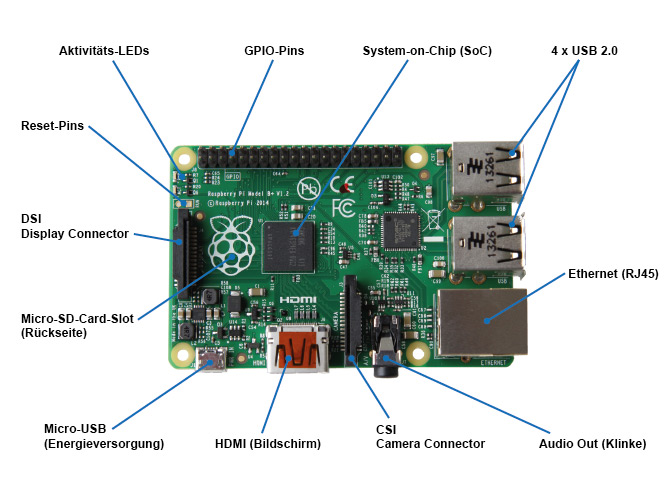
\includegraphics[width=9.5cm,height=4.2cm]{fig/Grundlagen/PIb+.jpg}
	\caption[Raspberry PI B+]{Raspberry PI B+\protect\footnotemark}
\end{figure}
\footnotetext{https://www.elektronik-kompendium.de/sites/raspberry-pi/bilder/19052513.jpg}
\newpage
\subsubsection{Verbinden mit einem PC}

Ben�tigt wird eine Ethernet-Verbindung zwischen Host und Raspberry Pi, die SD-Karte mit Image des verwendeten Betriebssystems Ubuntu und die Stromversorgung.

Auf das Raspberry Pi kann �ber mehrere M�glichkeiten zugegriffen werden.
Hierf�r sind die IP Konfigurationen des Pi�s und Hosts anzupassen (die IP vom Pi sollte unver�ndert sein).

Host-Ip:\newline
IP 192.168.22.160\newline
Maske: 255.255.255.0\newline
GW: 192.168.22.09

PI-IP:\newline
IP 192.168.22.161\newline
Maske: 255.255.255.0\newline

Die Login-Daten auf dem Raspberry lauten:\newline
User: pi\newline
Passwort: raspberry\newline

Testen Sie die Einstellungen indem sie das Raspberry Pi von dem jeweiligen verwendeten Host anpingen.

Nach erfolgreich ausgef�hrtem Ping-Befehl ist es nun m�glich, Programme oder Dateien mit dem Kommando scp an das Raspberry zu senden.

Folgende Schritte sind bei einem auftretenden Ping-Befehl-Fehler vorzunehmen:

Das Default Gateway muss zun�chst ermittelt werden, um die Ip-Einstellungen zu �ndern.

\begin{lstlisting}[language=bash]
sudo nano /etc/network/interfaces
\end{lstlisting}

Nun m�ssen noch die Einstellungen in der Datei \emph{/etc/network/interfaces} anpasst werden.

\begin{lstlisting}[language=bash]
sudo nano /etc/network/interfaces
\end{lstlisting}

Das ge�ffnete File sollte folgenderma�en aussehen:

\begin{lstlisting}[language=bash]
auto lo

iface lo inet loopback
iface eth0 inet static
address 192.168.22.161
netmask 255.255.255.0
gateway 192.168.22.9
#iface eth0 inet dhcp

allow-hotplug wlan0
iface wlan0 inet manual
wpa-roam /etc/wpa_supplicant/wpa_supplicant.conf
iface default inet dhcp
\end{lstlisting}

Das Interface eth0 ist eine statische Adresse mit der dargestellten IP, Maske und Gateway.
Ein Eintrag f�r das Routing ist vorzunehmen.

Der Netzwerkdienst muss neu gestartet werden, um die �nderungen �bernehmen zu k�nnen.

\begin{lstlisting}[language=bash]
sudo /etc/init.d/networking restart
\end{lstlisting}

\begin{lstlisting}[language=bash]
scp Quelle Ziel[USER@IP:PFAD]
scp RaspberryDemoUdpSendHost pi@192.168.22.161:/home/pi/
\end{lstlisting}

Es k�nnen auch Dateien vom PI auf den Host kopiert werden. Folgender Befehl kopiert die Datei \emph{file} vom Pi in das aktuelle Verzeichnis.

\begin{lstlisting}[language=bash]
scp pi@192.168.22.161:/home/pi/file .
\end{lstlisting}

\subparagraph{Benutzung eigener Monitor und Tastatur}
Es besteht die M�glichkeit �ber HDMI und USB einen Monitor und Tastatur anzuschlie�en. Hierf�r  muss die Netzwerkkonfiguration angepasst werden.


\subparagraph{�ber das Terminal}
Sie k�nnen sich �ber eine \emph{ssh} Verbindung auf das Raspberry Pi einloggen.
Sollte die Ip-Adresse des Raspberry ver�ndert worden sein, muss diese angepasst werden.
\begin{lstlisting}[language=bash]
ssh pi@192.168.22.161 
ssh USERNAME@IP
\end{lstlisting}

Die Eingabe des Passwortes des Benutzers \emph{pi} erfolgt �ber eine Blindeingabe.

\subsection{Peripherie}
\label{sec:hw-pher}

\subsubsection{Motoren}
Bei den Motoren handelt es sich um �ber Treiber "BL-Ctrl V1.2" gesteuerte Brushless DC Motoren "Robbe ROXXY BL-Outrunner 2824-34". Die Ansteuerung des Treibers erfolgt �ber den I2C Bus. An den Treiber werden 2 Byte Daten gesendet:
\begin{itemize}
	\item die I2C Adresse des gew�nschten Motors
	\item den PWM-Wert ( kleiner Wert langsam drehen, hoher Wert schnelles drehen)
\end{itemize} 

Der Treiber beh�lt die Werte 10 msec lang und verliert diese anschlie�end. Die Werte m�ssen also zyklisch gesendet werden.

Die Anzahl und Ordnung der Motoren ist je nach Typ des Helikopters unterschiedlich. Es gibt vier- oder acht Motorvarianten welche verschiedene Grundaufbauten haben k�nnen ( + oder x).

Der Code soll so allgemein gehalten werden, dass er f�r jeden dieser Typen verwendet werden kann. In der main.h wird mittels Definition angegeben f�r welchen Helikopter das Programm definiert werden soll. In der \emph{/hal/MOTOR/MOTOR.h} sind helikopterspezifische Daten abgelegt, darunter die I2C-Adressen jedes Motors, die Anzahl der Motoren, die min-Werte und max-Werte des PWM-Signales.

\subsubsection{Adafriut Ultimate GPS PI HAT\cite{doc:gpsHat}}
Dieses Modul wird direkt auf das PI aufgesteckt und leitet alle Pins bis auf die UART Pins weiter. Folgende Pins werden f�r das Bord ben�tigt und k�nnen nicht mehr verwendet werden:

\begin{table}[H]
	 \centering
	\begin{tabular}{|p{3cm}|p{11cm}| p{0.7cm} |}
		\hline 
		Pin &  Verwendung & Fest\footnotetext{Beschaltung kann nicht ge�ndert werden}\\ 
		\hline 
		UART TXD \newline UART RXD & Die einzige serielle Schnittstelle muss verwendet werden um mit dem GPS-Modul zu kommunizieren & \cmark \\ 
		\hline 
		GPIO \#4 &  Kann bei Bedarf verwendet werden, falls die Zeitsynchronisation mit dem Raspberry nicht ben�tigt wird& \xmark \\
		\hline
		EEDATA \newline EECLK & Werden f�r die Verbindung mit dem EEPROM ben�tigt, derzeit noch nicht vom Raspberry verwendet & \cmark\\
		\hline
	\end{tabular}
	\caption{Ultimate GPS Pins}
\end{table}

Dieses Modul liefert das GPS-Modul \textit{FGPMMOPA6H}(\href{https://www.adafruit.com/datasheets/GlobalTop-FGPMMOPA6H-Datasheet-V0A.pdf}{Datasheet}). Das Modul bietet Platz f�r eine Batteriezelle, f�r eine Real-Time-Clock und Prototypen Platz, um weitere Bauteile mittels L�ten hinzuzuf�gen. 

\subsubsection{ADS1015 12-Bit ADC\cite{doc:gpsADC}}

Hierbei handelt es sich um einen hochaufl�senden \href{https://www.adafruit.com/datasheets/ads1015.pdf}{12bit Analog-Digital-Konverter}. Der Konverter kann bis zu 3300 Umwandlungen in der Sekunde berechnen und besitzt eine I2C-Schnittstelle. Die Standardadresse des Bausteines ist die 7bit-Adresse 0x47. Diese Adresse kann durch die Verbindung folgender Pins mit dem \emph{ADDR-Pin} bei Bedarf angepasst werden: 
	
\begin{table}[H]
	\centering
	\begin{tabular}{|p{4cm}|p{4cm}| p{4cm} |}
		\hline 
		Adresse &  Pin 1 & ADDR\\ 
		\hline 
		0x48 &  GND &ADDR\\ 
		\hline 
		0x49 &  VDD & ADDR\\ 
		\hline 
		0x4A &  SDA & ADDR\\ 
		\hline 
		0x4B &  SCL & ADDR\\ 
		\hline 
	\end{tabular}
	\caption{ADC 12 Bit I2C Adress Manipulation}
\end{table}

Dieser ADC liefert folgende zwei verschiedene Betriebsmodi, welche �ber die Anschl�sse \emph{A0} bis \emph{A3} verwendet werden:


\begin{itemize}
	\item \emph{Single Ended}: berechnet den ADC der Spannung zwischen jedem der \emph{Ax-Pins} und Ground. Hiermit ist nur das Messen von positiven Spannungen m�glich. Effektiv verliert man dadurch ein Bit der Aufl�sung. Der Modus bietet doppelt so viele Inputs.
	\item \emph{Differential}: berechnet den ADC der Spannung zwischen \emph{A0} \& \emph{A1} und \emph{A2} \& \emph{A3}. Der Modus liefert weniger rauschanf�llige Signale.
\end{itemize}


Eine Spannung �ber 5V darf nicht angelegt werden, da diese das Modul zerst�ren w�rde.

\subsubsection{Pololu AltIMU-10 v4\cite{doc:imu}}

Dieses Modul besteht aus drei IC�s. Sie beinhalten die folgenden Funktionen:

\begin{table}[H]
	\centering
	\begin{tabular}{|p{4cm}|p{3cm}|p{4cm}|p{3.5cm}|}
	\hline
	 Funktion & IC & Default I2C Adresse  & Manipulate I2C  \\
	 \hline
	 Beschleunigungsmesser \newline  Magnetometer & \href{https://www.pololu.com/file/download/LSM303D.pdf?file_id=0J703}{LSM303D}  & 0x1D & 0x1E\\
	  \hline
	   Gyrometer &
	  \href{https://www.pololu.com/file/download/L3GD20H.pdf?file_id=0J731}{L3GD20H}& 0x6B& 0x6A \\
	  \hline
	 Barometer& \href{https://www.pololu.com/file/download/LPS25H.pdf?file_id=0J761}{LPS25H }& 0x5D & 0x5C \\
	 \hline 
	\end{tabular}
	\caption{IMU ICs}
\end{table}

Auch dieser Baustein verwendet zur Konfiguration und Kommunikation den I2C-Bus (7bit Adresse). Jeder dieser ICs besitzt eine eigene Adresse, die sich ebenfalls manipulieren l�sst, indem man den Pin \emph{SA0} auf \emph{GND} zieht.

\subsubsection{LIDAR-Lite v2\cite{doc:lidar}}

Dieser Lasersensor besitzt eine Reichweite bis zu $ 40 m$ mit einer Genauigkeit von $  \pm 0,025$ , eine Verz�gerung von 0,02 Sekunden und kann bis zu $500$ Messwerte pro Sekunde liefern. Der I2C-Bus kann mit $100kbits/s$ oder $400kbits/s$ betrieben werden. Eine eigene Adressierung ist m�glich. Als Standard-I2C Adresse ist die 0x62 festgelegt. Falls mehrere LIDAR Light v2 Sensoren an einem I2C-Bus h�ngen ist dies die Broadcast-Adresse.


\section{IDE}
\label{ide:ecl}

In der VM wird die IDE \emph{Eclipse} mit einem bereits installierten \emph{GCC} verwendet. Dieser \emph{GCC} kann f�r verschiedene Plattformen compilieren:
\begin{itemize}
	\item zum \emph{Native Compiler} (�bersetzt in den Maschinencode, der f�r die aktuelle Plattform ben�tigt wird)
	\item  zum \emph{Cross Compiler} (f�r die Verwendung um den Maschinencode f�r eine andere Plattform zu generieren) 
\end{itemize}

Das Storeage Passwort von Eclipse der VMware lautet:\newline
user\\
Das Storeage Passwort von Eclipse des Desktop-PC im EZS-Labor lautet:\newline
labor\\

\subsection{Compiler, Linker und Loader}

Beim Compilieren werden s�mtliche definierte Konstanten-, Makros- und Pr�prozessoranweisungen durch die angegebenen Werte ersetzt.

Der Compiler hat die Hauptaufgabe aus dem Quellcode (.c, .cpp und .h) in nativen Maschinencode zu �bersetzen. Der Maschinencode kann nur von einem bestimmten Prozessor gelesen werden. 
Ausnahmen hierbei sind z.B. Compiler in der .Net (C\#) Umgebung. Bei diesem werden die Source Dateien in sogenannte \emph{Intermedia Languages} �bersetzt, welche unabh�ngig vom Zielsystem sind. Bei der Ausf�hrung des Codes wird der \emph{Intermedia Languages} durch den Compiler bei jedem Start erneut in den prozessorspezifischen Maschinencode �bersetzt.

Weitere Aufgaben eines Compilers: 
\begin{itemize}
	\item Anzeige von Syntax Fehler und Warnungen
	\item Codeoptimierungen durchzuf�hren (verschiedene Stufen m�glich)
	\item Entfernen von Codesegmenten, die nie ausgef�hrt werden k�nnen
	\item Einf�gen von eigenen Funktionscode bei einem Funktionsaufruf
\end{itemize}

Als Ausgabe liefert der Compiler Code denn sogenannten Objekt Code.

Die einzelnen Objekt-Files m�ssen noch durch einen sogenannten Linker miteinander verbunden werden. Nach erfolgreicher Verbindung generiert der Linker die ausf�hrbare Datei.
Vom Linker werden unter anderem Funktionen aus der Standard Libary hinzugef�gt und alle Objektdateien, die noch nicht aufgel�ste Symbole enthalten, �berpr�ft und gel�st.
Man unterscheidet zwischen statischen und dynamischen linken. Das statische linken wird einmalig durchgef�hrt, dynamisches linken hingegen jedes mal zur Laufzeit.

Zuletzt gibt es noch den Loader. Dieser Loader l�dt Teile des ausf�hrbaren Codes, die in n�chster Zeit ben�tigt werden, in den Hauptspeicher.


\subsection{GNU Debugger GDB}

Der \emph{Gnu DeBugger} ist ein Standard Debugger von Linuxsystemen der die folgenden Sprachen unterst�tzt:
C, C++, Objective C, FORTRAN, Java, Pascal...

Neben den Standardaufgaben wie Stacktrace und Breakpoints setzen erm�glicht der GDB auch Manipulationen von Variablen w�hrend der Laufzeit des Programmes und Reverse Debugging.

F�r Eclipse ist ein PlugIn installiert, das den DBG zur Verf�gung stellt.

\subsection{Makefile}

Makefiles sind eine M�glichkeit (mittels des Programmes \emph{make}) um aus mehreren Quell-Files und Bibliotheken �ber Objekt-Files einen ausf�hrbaren Code zu generieren. Das Besondere an dieser Methode ist, dass beim Ausf�hren des Makefiles nur ge�nderte Quell-Dateien neu kompiliert werden m�ssen. Die daraufhin generierten Objekt-Files und   die unver�nderten Objekt-Dateien werden mit dem Linker neu verbunden. Beim herk�mmlichen Compilieren werden s�mtliche Quell-Dateien generiert und verbunden.
Kurz: es lassen sich Abh�ngigkeiten definieren. Dies ist zeitsparend, da nicht bei �nderung eines Files das komplette Projekt compiliert werden muss. Dies ist bei gro�en Projekten zu ber�cksichtigen.

Die Makefiles werden in einer Baumstruktur angelegt.

\paragraph{Bearbeitung von Makefiles}
F�r die Kompilierung neuer Source-Files m�ssen diese in den Makefiles bekanntgemacht werden und die �bersetzungs-Einstellungen bestimmt werden.

Zu bearbeiten sind im Trunk Ordner die Files  \emph{Makefile} und \emph{makeopts} und das jeweilige \emph{makefile} im Ordner, in dem eine neue Quelldatei hinzugef�gt wurde. F�r Host-Programme sind die files mit der Endung\emph{ -host} zu bearbeiten. �nderungen sind am Beispiel einer neuen c Source Datei \emph{MOTOR.c }im neu erstellen Ordner \emph{hal/MOTOR}.

Im \emph{trunk/Makefile} sind die Verweise auf alle anderen Makefiles aufgelistet. Dies ist das Root-Makefile.
Folgende �nderungen sind vorzunehmen:

\begin{lstlisting}[language=make]
product: ... MOTOR ...
\end{lstlisting}

F�r den Make all Befehl:

\begin{lstlisting}[language=make]
MOTOR:FORCE
cd hal/MOTOR; make all
\end{lstlisting}

F�r den Clean Befehl muss noch ein weiterer Eintrag erstellt werden.

\begin{lstlisting}[language=make]
cd hal/MOTOR; make clean
\end{lstlisting}

In dem \emph{trunk/makeopts} sind Einstellungen f�r das Makefile oder Generierung mit dem Makefile festgelegt. F�gen Sie die nachfolgende Zeile ein:

\begin{lstlisting}[language=make]
../hal/MOTOR/MOTOR.lib\
\end{lstlisting}

Zuletzt muss noch das Makefile im Ordner MOTOR erstellt und bearbeitet werden.
Dieses legt nun fest, welche Files f�r die Generierung verwendet werden sollen.
Hierf�r kopiert man am besten ein vorhandenes makefile um und �ndert anschlie�end die Zeilen, die aussagen welches \emph{.obj} und \emph{.lib} file zum kompilieren und builden verwendet werden soll.

\begin{lstlisting}[language=make]
OBJS= MOTOR.obj MOTOR1.obj
LIBRARY=MOTOR.lib
\end{lstlisting}

Sollten sich mehrere \emph{c} files im Ordner \emph{Motor} befinden, k�nnen diese durch einen Space getrennt angeben werden. Mit diesem Makefile wird aus \emph{MOTOR.C} wird das object file \emph{MOTOR.obj} generiert.

\subsection{Host Programme}
\label{sec:ide-host}

Um ein Project f�r eine Host-Anwendung zu erstellen, muss unter Eclipse ein neues \textit{ C/C++ Projekt }  mit dem Projekttyp \textit{ Executable Empty Projec t} und den Toolchains \textit{ Linux GCC } angelegt werden.

\subsection{Raspberry Pi Programme}
\label{sec:ide-pi}

Um ein Projekt f�r eine Raspberry Pi Remote-Anwendung zu erstellen, muss unter Eclipse ein neues \textit{ C/C++ Projekt }  mit dem Projekttyp \textit{ Executable Empty Project } und den Toolchains \textit{ Cross GCC } angelegt werden. 

Bei den Projekteigenschaften muss bei \textit{ C/C++ Build/Settings } beim Tool Settings der Cross Settings ausgew�hlt werden und der Prefix und Pfad zum verwendeten GCC angepasst werden.

Prefix: \textit{ arm-linux-gnueabihf- }

Pfad: \textit{ /home/user/rpi/tools/arm-bcm2708/gcc-linaro-arm-linux-gnueabihf-raspbian-x64/bin }

\paragraph{Debug Remote Einstellungen}

Bei  \textit{ Run as/Run Configurations } muss unter  \textit{ C/C++ Remmote Apllication } eine neue Konfiguration erstellt werden. Im Feld \emph{Projekt} die  Projektbezeichnung eingetragen. 

Unter \textit{ Remote Absolute File Path for C/C++ Application } wird der Pfad angegeben, in welchem die ausf�hrbare Datei gespeichert ist \newline (z.B. \emph{/home/ezs/git/helicopter-raspberry/NameDerAnwendung.elf})

Falls das Projekt neu gebaut werden muss sind die Target Einstellungen zu w�hlen.

Connection: Raspberry Target ausw�hlen.

Remote Absolute File Path for C/C++ Application: Hier den Pfad und Dateinamen angeben, in welchen die ausf�hrbare Datei gespeichert werden soll z.B. /home/pi/HELIKOPTER.elf

In das Feld  \textit{ Commands to execute before application } ist folgender Eintrag vorzunehmen: \newline
sudo -i \newline
chmod +x RaspberryDemoUdpReceiveTarget \newline
Dies macht das File zu einer ausf�hrbaren Datei und wird bei jedem Laden des Programmes auf das Raspberry Pi ausgef�hrt. 

Unter dem Reiter \emph{Debugger} ist das H�ckchen bei \emph{Stop on Starup at} zu setzen und in das daneben liegende Feld \emph{main} einzutragen. Dies sorgt daf�r das bei einem Programmstart automatisch ein Breakpoint bei Aufruf der Funktion Main erzeugt wird.

Bei Debugger Optionen ist der Pfad des GDB auf den \emph{gcc-linaro-arm-linux-gnueabihf-raspian-x64/bin/arm-linux-gnueabihf-gdb} 
und \emph{GDB command file} auf \emph{./gdbinit} zu �ndern. Der Debugger kann auf \href{https://github.com/raspberrypi}{GitHub} runtergeladen werden.

\subparagraph{Alternativ} kann auch der scp Befehl verwendet werden um die Datei auf das Raspberry Pi zu kopieren. \newline
scp ProgramName UserNameVonPi@IPAdressePi:SpeicherpfadAufPi \newline
Dann per ssh Zugriff, die Datei im angegeben Pfad zu einer ausf�hrbaren Datei machen und mit ./PfadZumFile.elf starten.
\subsection{Beispiel Code}
\label{sec:ide-example}

Anbei befinden sich zwei Codesegmente, die eine Nachricht �ber UDP/IP vom Raspberry Pi an den Host senden. Mit diesen Programmen k�nnen die zuvor beschriebenen Schritte zum Testen durchgef�hrt werden.

RaspberryDemoUdpSendHost.cpp:

\begin{lstlisting}[language=C++]{Name = RaspberryDemoUdpSendHost.cpp}
/*
* RaspberryDemoUdpSendHost.cpp
*
*  Created on: Oct 23, 2015
*      Author: Chris M�nch
*/

#include <iostream>
#include <stdio.h>
#include <sys/socket.h>
#include <netinet/in.h>
#include <string.h>
#include <unistd.h>

using namespace std;

int main(int argc, char * argv[]) {

cout << "Start\n";

int clientSocket, nBytesMessage, nBytesMessage2;
char message[12] = "Hello_World";
char message2[16] = "AnotherMessage";

nBytesMessage= sizeof(message)/ sizeof(message[0]);
nBytesMessage2 =sizeof(message2)/ sizeof(message2[0]);

struct sockaddr_in serverAddress;
socklen_t addressSize;

/*Create UDP socket*/
clientSocket = socket(PF_INET, SOCK_DGRAM, 0);

/*Configure settings in address struct*/
serverAddress.sin_family = AF_INET;
serverAddress.sin_port = htons(9999);
serverAddress.sin_addr.s_addr = htonl(INADDR_LOOPBACK);
memset(serverAddress.sin_zero, '\0', sizeof serverAddress.sin_zero);

/*Initialize size variable to be used later on*/
addressSize = sizeof(serverAddress);

printf("Start Sending Messages\n");

while(1){
sleep(1);
sendto(clientSocket,message,nBytesMessage,0,(struct sockaddr *)&serverAddress,addressSize);
sleep(1);
sendto(clientSocket,message2,nBytesMessage2,0,(struct sockaddr *)&serverAddress,addressSize);
printf("And send again....\n");
}

return 0;
}
\end{lstlisting}
RaspberryDemoUdpReceiveHost.cpp:

\begin{lstlisting}[language=C++]{Name = RaspberryDemoUdpReceiveHost.cpp}
/*
* RaspberryDemoUdpReceiveHost.cpp
*
*  Created on: Oct 23, 2015
*      Author: Chris M�nch
*/

#include <sys/types.h>
#include <sys/socket.h>
#include <netinet/in.h>
#include <arpa/inet.h>
#include <netdb.h>
#include <stdio.h>
#include <unistd.h>
#include <string.h>
#include <stdlib.h>
#include <errno.h>
#include <time.h>

#define LOCAL_SERVER_PORT 9999
#define BUF 255

using namespace std;

int main(int argc, char * argv[]) {
int s, rc, n;
socklen_t len;
struct sockaddr_in cliAddr, servAddr;
char puffer[BUF];
const int y = 1;
s = socket (AF_INET, SOCK_DGRAM, 0);
if (s < 0) {
printf ("%s: Kann Socket nicht �ffnen ...(%s)\n");
return 1;
}

/* Lokalen Server Port bind(en) */
servAddr.sin_family = AF_INET;
servAddr.sin_addr.s_addr = htonl (INADDR_ANY);
servAddr.sin_port = htons (LOCAL_SERVER_PORT);
setsockopt(s, SOL_SOCKET, SO_REUSEADDR, &y, sizeof(int));
rc = bind ( s, (struct sockaddr *) &servAddr,
sizeof (servAddr));
if (rc < 0) {
printf ("%s: Kann Portnummern %d nicht binden (%s)\n");
return 1;
}
printf ("%s: Wartet auf Daten am Port (UDP) %u\n",
argv[0], LOCAL_SERVER_PORT);
/* Serverschleife */
while (1) {
/* Puffer initialisieren */
memset (puffer, 0, BUF);
/* Nachrichten empfangen */
len = sizeof (cliAddr);
n = recvfrom ( s, puffer, BUF, 0,(struct sockaddr *) &cliAddr, &len );
if (n < 0) {
printf ("%s: Kann keine Daten empfangen ...\n",
argv[0] );
continue;
}

/* Erhaltene Nachricht ausgeben */
printf ("%s \n", puffer);

}
return 0;

}
\end{lstlisting}

\section{Git}

Git ist ein dezentrales Versionsverwaltungsprogramm. Es wird kein zentraler Server und es wird kein Internetzugang ben�tigt. Git ist komplett �ber die Kommandozeile Steuerbar, mittlerweile existieren aber auch viele Graphische Oberfl�chen f�r Git.

Das Paket wird mittels des Befehls
\begin{lstlisting}[language=bash]
sudo apt-get install git
\end{lstlisting}
installiert werden.

F�r das HElicopter Project existiert bereits ein Git-Repository. Dieses Repository wird von Herrn Agrawal verwaltet. F�r das Clonen und Pushen des verwalteten Quellcodes muss mit ihm Abgesprochen werden (Quelle/Ziel und Zugang).

Um Quellcode eines Repositorys zu klonen wird der folgende Befehl verwendet:

\begin{lstlisting}[language=bash]
git clone PfadDesRepositories SpeicherOrtDesRepositories
\end{lstlisting}

Als n�chstes sollte man Git bekannt machen wer man ist um zu erkennen wer welche �nderungen gemacht hat. Hierf�r geht man in das lokal heruntergeladene Repository Verzeichnis und setzt sich mit den folgenden Befahl seinen Namen und seine EMail Adresse:
\begin{lstlisting}[language=bash]
git config --global user.name MeinName
git config --global user.name MeineEMail@Mail.de
\end{lstlisting}
Diese Parameter sind bis zur einer �nderung in diesem lokalen Verzeichnis fest.

Anschlie�end sollte man sich einen Neuen Branch/Zweig erstellen auf welchem anschlie�end gearbeitet wird. Dies gelingt �ber das Kommando:
\begin{lstlisting}[language=bash]
git checkout -b MyOwnBranch
\end{lstlisting}
M�chte man auf einen anderen Branch wechseln muss folgender Befehl verwendet werden:
\begin{lstlisting}[language=bash]
git checkout AnotherBranch
\end{lstlisting}
Nat�rlich kann auch so auf ein anderes commit ge�nder werden.

Um Dateien oder ganze Verzeichnisse in das Quellverwaltung auszunehmen ist das Kommando
\begin{lstlisting}[language=bash]
git add filename.c
\end{lstlisting}
zu verwenden.

Um �nderungen des Repositorys lokal zu speichern wird das Kommando
\begin{lstlisting}[language=bash]
git commit -m "Message"
\end{lstlisting}
verwendet. Der Parameter -m sollte immer einen passenden Schl�ssigen Namen besitzen. Coder der commitet wird solle zuvor getestet werden oder zumindest keinen kompilerfehler liefern Auf andere commits kann jederzeit zugriffen werden. Mit dem Befehl
\begin{lstlisting}[language=bash]
git log 
\end{lstlisting}
werden alle commits und pushes angezeigt die auf die aktuelle lokale Version zutreffen. Mit den Information des Authoren und der Messsage des commits. 

Bearbeitete oder unversionierte Dateien lassen sich mit
\begin{lstlisting}[language=bash]
git status -u 
\end{lstlisting}
sichtbar machen.

Sollen Zwei Branches zusammengef�hrt werden m�ssen zun�chst s�mtliche Konflikte aufgel�st werden. Die �nderungen k�nnen mit
\begin{lstlisting}[language=bash]
git diff MyBranch TargetBranch
\end{lstlisting}
Angezeigt werden.

Mit dem Befehl
\begin{lstlisting}[language=bash]
git merge Targetbranch
\end{lstlisting}
wird der Branch in dem der Befahl aufgef�hrt, nach erfolgreicher Konflikt L�sung, wird mit dem angegeben TargetBranch Zusammengef�hrt.

\paragraph{Nach Pull Files alle als ge�ndert gekennzeichnet}

Direkt nach dem pull erfolgt eine �berpr�fung, ob der pull erfolgreich durchgef�hrt wurde. Falls der Fehler erst sp�ter erkannt wird, kann es zum Verlust von Daten kommen. Es empfiehlt sich eine tempor�re lokale Version abzuspeichern. Der Befehl
\begin{lstlisting}[language=bash]
git status -s
\end{lstlisting}
darf nichts zur�ckgeben, d.h. es gibt keine �nderungen im Vergleich zur Git Version. Wenn fehlerhafteiweise angezeigt wird, dass �nderungen vorgenommen wurden, wird mit
\begin{lstlisting}[language=bash]
git -diff
\end{lstlisting}
angezeigt, welche �nderungen vorgenommen wurden. Nun gibt es zwei verschiedene M�glichkeiten: Wenn ...
\subparagraph[... Steuerzeichen Controll M]{... Steuerzeichen Controll M}
hinzugef�gt worden ist, liegt es daran, dass die Files von einem anderen Betriebssystem aus bearbeitet wurden, z.B. von Windows zugegriffen wurde.

Bei Windows basierenden Systemen werden f�r ein Line Terminator (neuer Absatz und erste Position) zwei Steuerzeichen ben�tigt (\emph{Carriage Return} (ctrlM) und \emph{New Line Feed}(ctrlJ)). Bei Unix existiert nur das Steuerzeichen \emph{New Line Feed}. Das \emph{Carriage Return} besitzt keine spezielle Bedeutung in Linux basierenden Systemen. Daher wird das \emph{Carriage Return} nicht als Steuerzeichen erkannt und das Zeichen wird an jedes Zeilenende ins File hinzugef�gt. 

Mit dem Befehl \emph{dos2unix}, welcher eine File-Konvertierung von dos nach unix durchf�hrt, kann das Problem gel�st werden.

Zu beachten hierbei ist, dass die Konvertierung nur an ben�tigten Daten durchgef�hrt wird. Sonst k�nnte sie Verbindung mit Git zerst�rt werden.

Einzelne Files k�nnen wie folgt konvertiert werden:

dos2unix MAIN.c

Wenn mehrere Files konvertiert werden m�ssen, empfiehlt sich der Befehl find und dessen Ausgabe umzuleiten z.B:

find . -name *.c | xargs dos2unix

Der Befehl sucht alle Files im aktuellen Verzeichnis, die eine .c Endung im Namen tragen und konvertiert diese anschlie�end.

\subparagraph[... Keine Unterschiede]{... wenn keine Unterschiede}
in den Files angezeigt werden, m�ssen die folgenden Befehle ausgef�hrt werden (falls �nderungen vorgenommen wurden ist eine lokale Kopie zu erstellen, sonst sind die �nderungen gel�scht!):
\begin{lstlisting}[language=bash]
git rm --cached -r .

git reset ?-hard 
\end{lstlisting}
Dies l�scht rekursiv alle Dateiinhalte von dem Index. Anschlie�end wird der Index und der Working tree resetet. Jede �nderung seit dem letzen Commit werden r�ckg�ngig gemacht.

\section{Bekannte Probleme}
\subsection{Udp Socket Programm mit Windows 10 und VMware}
\label{vmWareError}

Wenn sich auf dem Host-System das Betriebssystem Windows 10 befindet, gibt es beim Empfangen der Udp-Packete Probleme. Der Programmcode ist voll funktionsf�hig. Dies kann man nachpr�fen indem man beide Programme in der VMware �ber die localhost Adresse laufen l�sst.

Die gesendeten Daten kommen nicht bei der VMware an. Au�erdem ist die VMware vom Pi nicht anzupingen, deshalb wurde die Firewall tempor�r deaktiviert. 
Daraufhin wurde der Ping Befehl erfolgreich ausgef�hrt. Die Daten kamen weiterhin nicht an.

Mit dem Tool Wireshark wurde mit aktiver und deaktivierter Firewall die Kommunikation mitgeschnitten. Bei deaktivierter Firewall kam die ICMP-Meldung, dass der Port nicht erreichbar ist.
Bei aktiver Firewall kamen diese Nachrichten nicht vor.

Daraufhin wurden f�r die Firewall Ausnahmen generiert, das jegliche Kommunikation von der IP des Raspberry Pi auf den Port 9999 ankommt und nicht blockiert wird.

Da dies ebenfalls keine Auswirkung hat, wird wohl noch in einem von Windows bereitgestellten Dienst/Service die Kommunikation verhindert. Auf Funktion mit einem anderen Windows Betriebssystem k�nnen keine Annahmen getroffen werden.

Mit einem Linux/Ubuntu System funktionieren die Programme fehlerfrei.

Als Ausweichm�glichkeit wurde ein PC f�r folgende Arbeit in der Hochschule bereitgestellt.

\chapter{Realisierung}
\label{sec:real}

Die Hardware kann bei Bedarf in einem abschlie�barem Container gelagert werden und nach Absprache mit Projektteilnehmer und Projektleiter die Hardware auch mitgenommen werden. 

\section{Inbetriebnahme der Hardware}
\label{Inbetriebname}
Eine MicroSD-Karte mit aufgespieltem Ubuntu-Image muss in den Raspberry Pi Kartenslot gesteckt werden.

Als Versorgungsspannung benötigt der Quadrocopter 11.7 Volt mit Akku oder 10V-11V mit Netzger�t. Beim Umlegen des Hauptschalters sollen die LED�s am Quadrocopter und PI blinken sowie die Motoren einen Impuls erhalten.

Beim Motorentests sollte der Quadrocopter befestigt werden, damit dieser nicht besch�digt wird geht. Im EZS-Labor wurde hierf�r an einem Arbeitsplatz ein Schraubstock montiert.

Der I2C-Bus (braunes rot/blaues Kabel) wird mit den I2C Pins des Raspberry PI B+ verbunden. Pin2 ist Serial Data und Pin5 ist Serial Clock. Braun-blaues Kabel ist f�r das Clocksignal , braun-rotes Kabel ist f�r das Datensignal. Testen kann man die I2C Configuration des PI mit dem Befehl:

sudo i2cdetect -y 1

In der nachfolgenden Tabelle finden sich alle beinhalteten Komponenten des I2C1-Buses wieder.
\begin{table}[H]
	\begin{center}
		\begin{tabular}{| l | p{3cm} | |p{5cm}|}
			\hline
			Typ & I2C Adresse 7bit  & Information \\
			\hline
			ADC & 0x49 & ADDR <-> VDD\\
			\hline
			Beschleunigungssensor  \newline  Magnetometer & 0x1E  & SA0 <-> GND  \\
			\hline 
			Barometer & 0x5C & SA0 <-> GND \\
			\hline 
			Gyrometer & 0x6A & SA0 <-> GND\\
			\hline
			Brushless Motoren Treiber 1-4  &0x29,0x2A, 0x2B,0x2C& Je nach HElicopter Typ unterschiedlich, I2C Adressen sind per HW festgelegt , per Software nicht �nderbar\\
			\hline 
			Brushless Motoren Treiber 5-8  & 0x5A,0x5C, 0x5E,0x60& Nicht getestet, zu �berpr�fen und ggf. zu �berarbeiten in der \textit{MOTOR.h}\\
			\hline
			Laser Sensor & 0x62 & Standardadresse des Herstellers\\
			\hline
		\end{tabular}
	\end{center}
	\caption{I2C Adsressvergabe}
\end{table}




\paragraph{Der Remoteempf�nger GR-16} hat drei Verbindungen zum Raspberry Pi:
Eine 3,6V bis 8,4V Spannungsversorgung, Ground und eine Datenverbindung.
\phantomsection
\label{Receiver}
\begin{figure}[H]
	\centering
	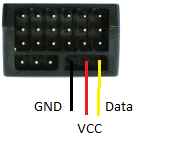
\includegraphics{fig_motor/GR-16.png}
	\caption[GR-16 Verkabelung]{GR-16 Verkabelung\protect\footnotemark}
\end{figure}
\footnotetext{http://www.graupner.de/mediaroot/files/33508\_Kurzanleitung\_de.pdf}
Die Spannung und Ground kann direkt �ber das Raspberry Pi bezogen werden. F�r die Daten muss einer der GPIO Pins als Input deklariert werden.

Um die Fernbedienung mx-20 mit dem Empf�nger GR-16 zu verbinden m�ssen beide Ger�te eingeschaltet sein (Empf�nger LED blinkt Rot). Beim Anschalten der Fernbedienung wird gefragt ob \emph{HF} EIN oder AUS ist. Stellen Sie auf AUS und best�tigen Sie mit Dr�cken der Set-Taste. Dr�cken sie erneut Set um in die Einstellungen zu gelangen. Scrollen Sie sich mit den Pfeiltasten durch das Men� bis Sie das Men� \emph{Grundeinstellungen Mod.} sehen. �ffnen Sie mit Set das Men� und scrollen Sie durch bis zu Punkt \emph{Modul}. Best�tigen Sie noch NICHT mit der Set-Taste. 
Halten Sie nun am Empf�nger solange die Set Taste gedr�ckt, bis sich zur der roten LED noch eine gr�ne LED einschaltet. Bet�tigen Sie jetzt den Set-Taster auf der Fernbedienung. Es sollte der Info-Text \emph{Binden ...} angezeigt werden.
Wenn die Verbindung erfolgreich durchgef�hrt wurde leuchtet die LED dauerhaft gr�n. \cite{doc:gt-16}

\newpage

\section{Debuggen der Programme}

\paragraph{Target laden}
Rechtsklick auf Projekt Ordner, \newline
Build Configurations -> Set Active -> Target.\newline
Rechtsklick auf Projekt Ordner, Build Project.

Debug Pfeil anklicken und helicopter-raspberry target ausw�hlen.

Oder �ber das Terminal: In das Verzeichnis \emph{helikopter-raspberry/impl/trunk/} wechseln
und mit dem Befehl \newline
\emph{make MAKECMDGOALS=target}\newline
das Programm  kompilieren und automatisch auf das Raspberry Pi laden.

\paragraph{Host laden}
Rechtsklick auf Projekt Ordner, 
Build Configurations -> Set Active -> Host.
Rechtsklick auf Projekt Ordner, Build Project.

Debug Pfeil anklicken und READ-UDP ausw�hlen.

\paragraph{Programme laufen lassen}
In die Debug-Ansicht von Eclipse wechseln (oben rechts). In dem Debug-Fenster sollten nun eine Remote-Anwendung (Anwendung auf Pi) und eine Host-Anwendung gestartet sein. Um diese laufen zu lassen muss der jeweilige Prozess ausgew�hlt werden und auf Resume geklickt werden sowie ggf. Breakpoints entfernt werden.

Nachdem die beiden Programme laufen muss noch der zu startende Testfall ausgew�hlt werden. Dies geschieht, in dem man �ber die Console die jeweiligen Testfall ausw�hlt, z.B. "testmatlabimu". Das im Grundlagenteil Udp-Programm ist hier als Testfall eingef�gt und kann mit der Eingabe "testudp" gestartet werden.

Nun laufen die Programme. Falls im ausgew�hlten Testfall Ausgaben vorhanden sind, sind diese in der Console zu sehen.

\paragraph{Beenden der Applicationen}
Um Probleme zu vermeiden ist es wichtig, die laufenden Programme immer manuell anzuhalten und zu \emph{killen}. Dies gelingt, in dem man in der Debug-Ansicht auf das zu beendene Programm rechtsklickt und auf Terminate klickt. 

\paragraph{Testf�lle}
In der main.c wird in dem definiertem \emph{enum} enumTestCases ein neuer Testfall angelegt.
In der int main(){...} wird bei Start auf eine Eingabe des zu startenden Testfalles gewartet. Hier muss noch ein \emph{else if}-Anweisung erg�nzt werden. 
In der Variable runCommand wird der Name des abzuarbeitenden Testfalles abgespeichert.
In der nachfolgenden \emph{Switch}-Anweisung steht der eigentliche Code, welcher bei Auswahl dieses Testfalles ausgef�hrt wird.

\newpage
\section{Umstellung auf eine automatische dynamische Testumgebung}

Die Main-Funktion zum Testen soll umstrukturiert werden, da die vorherige Struktur recht umst�ndlich zu testen und zu bedienen war. Es muss vor jedem einzelnen Testfall das Programm komplett auf das Raspberry �bertragen werden und �ber die Remote-Verbindung der zu startende Testfall h�ndisch ausgew�hlt werden. Dieser wird ausgef�hrt und das Programm ist beendet, sobald der Testfall beendet ist. Um einen weiteren Test zu starten musste wieder eine Remote-Verbindung aufgebaut werden. Dies funktioniert, ist aber nicht die optimale L�sung.

Stattdessen soll die neue Main-Funktion �ber eine Dauerschleife verf�gen, in dieser ein Textfile ausgelesen wird. Dieses File beinhaltet die zu startenden Testcases des Programmes.

In diesem Textfile werden alle Testf�lle festgehalten, mit einem Status ob dieser laufen soll oder nicht. Der Status soll w�hrend der Laufzeit des Programmes �nderbar sein und dieses auch nicht unterbrechen.

Dieses Textfile sieht folgenderma�en aus:

...\\
testmotorpwm=1\\
testmotorisr=1\\
testmotortxt=0\\
....\\

Dies bedeutet: die Testf�lle testmotorpwm und testmotorisr sollen gestartet werden, testmotortxt soll nicht gestartet werden.
Der Testfall testmotorpwm wird zuerst ausgelesen und von der Main-Funktion auf Null zur�ckgesetzt. Anschlie�end l�uft der Testfall ab.

W�hrenddessen wird der Testfall testmotortxt aktiviert. 

...\\
testmotorpwm=0\\
testmotorisr=1\\
testmotortxt=1\\
....

Ist der Testfall beendet wird das Textfile erneut eingelesen und der n�chste gesetzte Testfall wird gestartet.

\newpage
\paragraph{Umstrukturierung der main.c:}

Es wurde eine Endlosschleife eingef�gt. Statt auf eine Tastatureingabe �ber eine Konsole zu warten, wird in dieser alle zwei Sekunden das \textit{\_Testfile} ausgelesen und �berpr�ft, ob ein Testfall ausgef�hrt werden soll.


In allen Testf�llen darf keine Endlosschleife vorhanden sein, bzw. muss in weiteren Endlosschleifen ein Abbruchkriterium festgelegt sein. In den meisten F�llen kann der Testfall mit Dr�cken der Taste \textit{p} abgebrochen werden. In Testf�llen, in denen ein Testfile ausgelesen wird, wird bei Erreichen des Dateiendes der Testfall beendet und gelangt so wieder in die Hauptschleife zur�ck.

\paragraph{Script zum Setzen der Testf�lle:}

Zum Setzen oder L�schen eines Testfiles wurde ein Script geschrieben, welches auf das textfile \textit{\_Testfile} zugreift und die Eintr�ge je nach Eingabe �berarbeitet.

Verwendet wird das Script folgenderma�en:

\begin{lstlisting}[language=bash]
.\testcase NameTestfall [Modus]
\end{lstlisting}
 	 
Als ersten Parameter ist der zu �berarbeitende Testfall anzugeben.\\
Der Modus ist ein optionaler Parameter. Ist dieser Parameter nicht vorhanden, wird automatisch \emph{set} angenommen. \textit{set} markiert den Testfall als abzuarbeiten, \textit{clear} l�scht diese Markierung wiederrum. Das Script zeigt keinen Fehler oder Warnung auf, wenn der testcase nicht gelistet ist.

Der Quellcode ist im Kapitel \ref{script_testcase} \nameref{script_testcase} auf S.\pageref{script_testcase} einzusehen.

\newpage
\section{Valedierung der empfangenen Werte}
\label{sec:real-unter}
Im testcase testmatlabimu stimmen die empfangenen und gesendeten Werte nicht �berein. Hier ist der Fehler zu finden und zu beheben.

Es werden insgesamt 11 double Values von den diversen Sensoren an den Host gesendet. Die Kalkulation der Werte ist richtig, kommen jedoch beim Empf�nger falsch an. Dieses Fehlverhalten gilt es zu untersuchen.

Hierf�r wurde ein neuer Testfall angelegt, alle 11 Double Werte per UDP versendet und diese auf beiden Seiten ausgegeben. 

Nach dem Setzen der Breakpoints, so das nur einmal die Werte gesendet werden, erhalten wir folgende Ausgaben auf der Console:

\begin{multicols}{2}
	 \begin{lstlisting}[language=C++]
	 Starting read over UDP
	 /home/ezs/git/helikopter- raspberry/impl/trunk/host /READ-UDP.elf: Wartet auf Daten am Port (UDP) 5000
	 Acc X 0.000000 
	 Acc Y 0.910135 
	 Acc Z -0.488599 
	 Mag X -10.533617 
	 Mag Y 0.000024 
	 Mag Z 0.000021 
	 Gyro yaw 0.000014 
	 Gyro pitch -0.473037 nGyro roll 0.473037 
	 Temp -0.396741 
	 Press 31.825000 
	 \end{lstlisting}
	
	\columnbreak
	
	 \begin{lstlisting}[language=C++]
	 Received string is testallsensordata 
	 Starting IMU Matlab Test
	 
	 
	 Acc X 0.910135 
	 Acc Y -0.488599 
	 Acc Z -10.533617 
	 Mag X 0.000024 
	 Mag Y 0.000021 
	 Mag Z 0.000014 
	 Gyro yaw -0.473037 
	 Gyro pitch 0.473037 
	 Gyro roll -0.396741 
	 Temp 31.825000 
	 Press 987.931396 
	 \end{lstlisting}
\end{multicols}
 

Nach einem Vergleich f�llt auf, dass beim Empfang der Daten sich bei X-Wert vom Acc eine Null eingef�gt hat. Ansonsten scheinen die Daten zu stimmen. Die Daten sind nur um eins versetzt.

In der read-udp-host.c werden die Werte in der Variable \emph{l\_recvImuState\_st} gespeichert. Beim Betrachten der Inhalte dieser Variablen ist zu erkennen, dass diese in \emph{acc.f64} einen Wert hat der Circa null entspricht, die restlichen Werte sehen richtig aus, nur weiterhin um einen Wert verschoben.

Verdacht: Beim Senden der Daten wird auch noch ein Zeitstempel dieses Telegramms mitgesendet: 
\begin{lstlisting}[language=C++]
//time.h
struct timespec{
	__time_t tv_sec; /* Seconds */
	__syscall_slong_t tv_ns	/* Seconds */
	};

//udpImuLib.c
struct timespec l_timespec_st;

\end{lstlisting}

Diese Daten haben die L�nge von 8 Byte (beide vom Typ long int). Diese Daten werden mit den Sensordaten gesendet. Die Paketl�nge nimmt zu.
Da auf der Empf�ngerseite die Empfangsstruktur aber diesen timestamp nicht erwartet, geht er davon aus, dass der erste Wert, den er bekommt, f�r den Acc X Sensor-Wert steht.
Aus diesem Grund verrutschen die restlichen Daten um eins ab und der erste Sensor-Wert ist falsch da dieser den Timestamp widerspiegelt.

\paragraph{Problembehebung}
Die fehlenden Daten m�ssen in dem Struct bekannt gemacht werden, sodass die L�nge der beiden Felder nun gleich Gro� sind (96 Byte).
Hierf�r musste das Struct \emph{halImu\_orientationValues} im imu.h um einen Datentyp struct timespec erweitert werden sowie die notwendige Standardlibary \emph{time.h} hinzugef�gt werden.
Dann wurde die Testausgabe um den Timestamp erweitert.
Die Werte stimmen nun �berein:
\begin{multicols}{2}
	\begin{lstlisting}[language=C++]
	Starting read over UDP
	/home/ezs/git/helikopter -raspberry/impl/trunk/host /READ-UDP.elf: Wartet auf Daten am Port (UDP) 5000
	Time  1434105267.000000000 
	Acc X 0.792776 
	Acc Y -0.555661 
	Acc Z -10.581519 
	Mag X 0.000024 
	Mag Y 0.000021 
	Mag Z 0.000014 
	Gyro yaw -0.228889 
	Gyro pitch -0.122074 
	Gyro roll -0.488296 
	Temp 32.056250 
	Press 987.923828 
	\end{lstlisting}
	\columnbreak
	\begin{lstlisting}[language=C++]
	 Received string is testallsensordata 
		Starting IMU Matlab Test
		 
	
	
	Acc X 0.792776 
	Acc Y -0.555661 
	Acc Z -10.581519 
	Mag X 0.000024 
	Mag Y 0.000021 
	Mag Z 0.000014 
	Gyro yaw -0.228889 
	Gyro pitch -0.122074 
	Gyro roll -0.488296 
	Temp 32.056250 
	Press 987.923828 
	\end{lstlisting}
\end{multicols}

\begin{lstlisting}[language=C++]
#include <time.h>
typedef struct{
	struct timespec l_timestamp_st;
	halAccmag_3dDoubleVector acc;
	halAccmag_3dDoubleVector mag;
	strGyro gyro;
	double temperature_f64;
	double pressure_f64;
} halImu_orientationValues;

\end{lstlisting}

\section{Software Motortreiber}

Es soll Software f�r den Hardware-Treiber, der die Motoren ansteuert, geschrieben werden. Zun�chst muss der Raspberry Pi mit dem I2C-Bus verbunden werden. 
Die I2C Adressen der Motoren sind in der Motor.h hinterlegt. F�r die Quadrocopter wurden die Werte definiert. Die Werte des Octocopter m�ssen zun�chst �berpr�ft werden.

Mittels des Befehl:

\begin{center}
	i2cdetect -y 1
\end{center}

k�nnen die vergebenen Adressen im Bussystem angezeigt und validiert werden.

Die Daten, die von dem Hardware Brushless-Controller erwartet werden, besitzen folgendes Format:

	\begin{table}[H]
		\centering
		\begin{tabular}{|c|c|}
			\hline
			I2C Adresse [1 Byte] & PWM Value [1 Byte]\\ \hline
		\end{tabular}
	\caption{I2C Frame Brushless Motoren Treiber}
	\end{table}

Mit Hilfe des Befehls 

\begin{center}
	i2cset -y 1 0x29 0x55
\end{center}

wird an den Controller mit der I2C Adresse 0x29 ( Motor Nr.1) der Wert 0x55 gesendet.

\subsection{Verwendung des Software-Treibers}

In der main.h muss zun�chst definiert werden, auf welchem Typ von den HElicoptern das Programm geladen werden soll.
\begin{lstlisting}[language=C++]
#include <time.h>
#define Quadro_Plus 1
//#define Quadro_X 1
//#define Okto_Plus 1
\end{lstlisting}

Anschlie�end sollte baldm�glichst die InitMotor() aufgerufen werden, die unter anderem einen Timer initialisiert und startet. Bei Ablauf des Timers wird ein Flag gesetzt. Dieses Flag muss im Quellcode mit der Funktion \emph{GetFlagRunSendPwmToMotor()} abgefragt werden. Wenn dieses Flag gesetzt ist, muss die Funktion \emph{sendPwmToMotor()} aufgerufen werden.

\begin{lstlisting}[language=C++]
...
InitMotor();
...
while(1){
...
if(GetFlagRunSendPwmToMotor() == 1){
sendPwmToMotor();
}
...

}
\end{lstlisting}
Der aktuelle PWM-Wert eines Motors kann mittels der Funktion \emph{GetPwmMotor(...)} zur�ckgegeben werden.

\begin{lstlisting}[language=C++]
value = GetPwmMotor(6);
value > 0? value--: (value=DEFMotorSetpointMIN);
SetPwmMotor(DEFMotorNo7_PWM, value ,0);
\end{lstlisting}

Wichtig: Alle ISR sollen knapp gehalten werden, da ansonsten die Motoren nicht mehr angesprochen werden k�nnen.

Mit der Funktion \emph{SetPwmMotor(...)} k�nnen die PWM-Werte, die  per I2C gesendet werden, �berschrieben werden. Optional kann ein Flag gesetzt werden. Ist dies der Fall wird anschlie�end die Funktion \emph{sendPwmToMotor()} aufgerufen.

\subsection{Headerfile}

Hier sind die verschiedenen HElicopter Varianten sowie deren definierte Eigenschaften (Anzahl Motoren, Drehrichtung der Motoren, Motorenreihenfogen) festgehalten.

F�r weitere Informationen (wie z.B. Namen der defines) siehe in Kapitel \ref{motorH} in  \nameref{motorH} auf S.\pageref{motorH} .

\subsection{Funktionen}

Beschreibung der Funktionen befinden sich in den jeweiligen dar�ber liegenden Kommentaren mit Parametern und Return Values.

Auf alle globalen Variablen/Flags werden mit Funktionen zugegriffen. Ein direkter Zugriff ist zu vermeiden.

\begin{lstlisting}[language=C++,firstnumber=14]
/* Global Variables */
char BLCtrlADRExecuteOrder[DEFMotorsCount];
char PWMValue[DEFMotorsCount];

//Flags
char flagRunSendPwmToMotor;
\end{lstlisting}

\begin{lstlisting}[language=C++,firstnumber=21]
/*!***************************************************************
* \author Chris Mönch( chmoit00 )
*
* \brief calls init functions which needed for the motor driver:
* SetFlagRunSendPwmToMotor(0);
*	SetMotorExecutionOrder();
*	SetPwmMotor(DEFMotorALL_PWM, DEFMotorSetpointMIN, 0);
*	Last one always initMotorTimer()
*	InitMotorTimer(microSeconds);
*	SetFlagRunSendPwmToMotor(1);
*
* \param[ in ] microSeconds - Time in uS when Timer expired.
*
* \internal
* CHANGELOG:
*
* \endinternal
*****************************************************************/
void InitMotor(int microSeconds){
	SetFlagRunSendPwmToMotor(0);
	SetMotorExecutionOrder();
	SetPwmMotor(DEFMotorALL_PWM, DEFMotorSetpointMIN, 0);
	//Last one always initMotorTimer()
	InitMotorTimer(microSeconds);
	SetFlagRunSendPwmToMotor(1);
}
\end{lstlisting}

\begin{lstlisting}[language=C++,firstnumber=48]
/*!***************************************************************
* \author Chris Mönch( chmoit00 )
* \date 2016/01/08
*
* \brief set Motor Exectution Order
*
* \internal
* CHANGELOG:
*
* \endinternal
*****************************************************************/
void SetMotorExecutionOrder(){
	GetBLCtrlADRExecuteOrder(&BLCtrlADRExecuteOrder[0]);
}
\end{lstlisting}

\begin{lstlisting}[language=C++,firstnumber=63]
/*!***************************************************************
* \author Chris Mönch( chmoit00 )
* \date 2016/01/08
*
* \brief sets PWM Signal of selected Motor to pwmValue
* \details toSet = 00001111 sets the first 4 Motors in Execution Order to pwmValue
*
* \param[ in ] toSet - Which Motor to Set
* \param[ in ] pwmValue - Which Value so Set
* \param[ in ] forceSend - optional Parameter if !0 flagRunSendPwmToMotor will be set
*
* \internal
* CHANGELOG:
*
* \endinternal
*****************************************************************/
void SetPwmMotor(char toSet , int pwmValue, int forceSend){
	int i=0;
	pwmValue = pwmValue >= DEFMotorSetpointMIN ? pwmValue :  DEFMotorSetpointMIN;
	pwmValue = pwmValue <= DEFMotorSetpointMAX ?  pwmValue :  DEFMotorSetpointMAX;
	while(toSet != 0 && i < DEFMotorsCount){
	
		if(toSet%2){
			PWMValue[i]= pwmValue;
		}
		toSet= toSet >>1;
		i++;
	}
	if(forceSend != 0){
		SetFlagRunSendPwmToMotor(1);
	}
}
\end{lstlisting}

\begin{lstlisting}[language=C++,firstnumber=96]
/*!***************************************************************
* \author Chris Mönch( chmoit00 )
* \date 2016/01/08
*
* \brief adds to the current PWM Signal of selected Motor the pwmValue
* \details toSet = 00001111 add to the first 4 motors pwmValue
*
* \param[ in ] toSet - Which Motor to Set
* \param[ in ] pwmValue - adding pwm value to current PWMValue
* \param[ in ] forceSend - optional Parameter if !0 flagRunSendPwmToMotor will be set
*
* \internal
* CHANGELOG:
*
* \endinternal
*****************************************************************/
void AddPwmMotor(char toSet , int pwmValue, int forceSend){
	int i=0;
	
	while(toSet != 0 && i < DEFMotorsCount){
	
		if(toSet%2){
			pwmValue = pwmValue+GetPwmMotor(i);
			pwmValue = pwmValue >= DEFMotorSetpointMIN ? pwmValue :  DEFMotorSetpointMIN;
			pwmValue = pwmValue <= DEFMotorSetpointMAX ?  pwmValue :  DEFMotorSetpointMAX;
			PWMValue[i]= pwmValue;
		}
		toSet= toSet >>1;
		i++;
	}
	if(forceSend != 0){
		SetFlagRunSendPwmToMotor(1);
	}
}

\end{lstlisting}

\begin{lstlisting}[language=C++,firstnumber=131]
/*!***************************************************************
* \author Chris Mönch( chmoit00 )
* \date 2016/01/08
*
* \brief Subtract to the current PWM Signal of selected Motor the pwmValue
* \details toSet = 00001111 subtract to the first 4 motors pwmValue
*
* \param[ in ] toSet - Which Motor to Set
* \param[ in ] pwmValue - pwm value to subtract from Current PWMValue
* \param[ in ] forceSend - optional Parameter if !0 flagRunSendPwmToMotor will be set
*
* \internal
* CHANGELOG:
*
* \endinternal
*****************************************************************/
void SubbPwmMotor(char toSet , int pwmValue, int forceSend){
	int i=0;
	
	while(toSet != 0 && i < DEFMotorsCount){
	
		if(toSet%2){
			pwmValue = GetPwmMotor(i)- pwmValue;
			pwmValue = pwmValue >= DEFMotorSetpointMIN ? pwmValue :  DEFMotorSetpointMIN;
			pwmValue = pwmValue <= DEFMotorSetpointMAX ?  pwmValue :  DEFMotorSetpointMAX;
			PWMValue[i]= pwmValue;
		}
		toSet= toSet >>1;
		i++;
		}
	if(forceSend != 0){
		SetFlagRunSendPwmToMotor(1);
	}
}
\end{lstlisting}

\begin{lstlisting}[language=C++,firstnumber=167]
/*!***************************************************************
* \author Chris Mönch( chmoit00 )
* \date 2016/01/08
*
* \brief Gets pwmValue from a specific motor
* \details
*
* \param[ in ] motorNumber - which motor
*
* \param[ out ] pwmValue of the chosen Motor, returns O if chosen Motor not exist in these HElicoptertype
* 
* \internal
* CHANGELOG:
*
* \endinternal
*****************************************************************/
int GetPwmMotor(int motorNumber){
	return motorNumber < DEFMotorsCount ? PWMValue[motorNumber]: 0;
}
\end{lstlisting}

\begin{lstlisting}[language=C++,firstnumber=188]
/*!***************************************************************
* \author Chris Mönch( chmoit00 )
* \date 2016/01/08
*
* \brief init Timer for the IsrMotor
* \details
*
* \param[ in ] microSeconds - Time in uS when Timer expired.
*
* \internal
* CHANGELOG:
*
* \endinternal
*****************************************************************/
void InitMotorTimer(int microSeconds){

	struct sigaction sa;
	struct itimerval timer;
	
	//Creates Signal, if signal Rising a_handler called
	memset(&sa, 0 , sizeof(sa));
	sa.sa_handler = &IsrSetFlag;
	sigaction(SIGVTALRM, &sa, NULL);
	
	//Expire the Timer after:
	timer.it_value.tv_sec = 0;
	timer.it_value.tv_usec = 0;
	//And every ... after that:
	timer.it_interval.tv_sec = 0;
	timer.it_interval.tv_usec = microSeconds;
	//upon expiration the signal SIGVTALRM raised
	setitimer(ITIMER_VIRTUAL, &timer , NULL);
}
\end{lstlisting}

\begin{lstlisting}[language=C++,firstnumber=222]
/*!***************************************************************
* \author Chris Mönch( chmoit00 )
* \date 2016/01/08
*
* \brief set flag flagRunSendPwmToMotor
*
* \param[ in ] 1 Set Flag, else clear Flag
*
* \internal
* CHANGELOG:
*
* \endinternal
*****************************************************************/
void SetFlagRunSendPwmToMotor(char value){
	if(value == 1){
		flagRunSendPwmToMotor=value;
	}else{
		flagRunSendPwmToMotor=0;
	}
}
\end{lstlisting}

\begin{lstlisting}[language=C++,firstnumber=243]
/*!***************************************************************
* \author Chris Mönch( chmoit00 )
* \date 2016/01/08
*
* \brief ISR for set flag as flagRunSendPwmToMotor
*
* \internal
* CHANGELOG:
*
* \endinternal
*****************************************************************/
void IsrSetFlag(){
	flagRunSendPwmToMotor=1;
}
\end{lstlisting}

\begin{lstlisting}[language=C++,firstnumber=258]
/*!***************************************************************
* \author Chris Mönch( chmoit00 )
* \date 2016/01/08
*
* \brief get flag flagRunSendPwmToMotor
*
* \param[out] flag flagRunSendPwmToMotor
*
* \internal
* CHANGELOG:
*
* \endinternal
*****************************************************************/
char GetFlagRunSendPwmToMotor(){
	return flagRunSendPwmToMotor;
}
\end{lstlisting}

\begin{lstlisting}[language=C++,firstnumber=275]
/*!***************************************************************
* \author Chris Mönch( chmoit00 )
* \date 2016/01/08
*
* \brief sends every timer interrupt to the motors the specific pwm values
*
* \internal
* CHANGELOG:
*
* \endinternal
*****************************************************************/
void sendPwmToMotor(){
	int i;
	for(i = 0; i < DEFMotorsCount ;i++)
	{
		g_lldI2c_WriteI2c_bl(BLCtrlADRExecuteOrder[i],&PWMValue[i],1);
	}
}
\end{lstlisting}

\begin{lstlisting}[language=C++,firstnumber=294]
/*!***************************************************************
* \author Chris Mönch( chmoit00 )
* \date 2016/01/08
*
* \brief Get the I2C addresses orderd by execution (defined in MOTOR.h)
* \details
*
* \param[ in ] Array where the I2C Addresses will be stored
*
* \internal
* CHANGELOG:
*
* \endinternal
*****************************************************************/
void GetBLCtrlADRExecuteOrder(char BLCtrlADRExecuteOrder[]){
#if defined(Quadro_X) || defined(Quadro_Plus)
int BLCTRLADR[4] = {DEFMotorNo1_BLCtrlADR, DEFMotorNo2_BLCtrlADR, DEFMotorNo3_BLCtrlADR, DEFMotorNo4_BLCtrlADR};

BLCtrlADRExecuteOrder[DEFMotorNo1_OrderIDX ]=BLCTRLADR[0];
BLCtrlADRExecuteOrder[DEFMotorNo2_OrderIDX]=BLCTRLADR[1];
BLCtrlADRExecuteOrder[DEFMotorNo3_OrderIDX]=BLCTRLADR[2];
BLCtrlADRExecuteOrder[DEFMotorNo4_OrderIDX]=BLCTRLADR[3];

#endif

#ifdef Okto_Plus
int BLCTRLADR[8] = {DEFMotorNo1_BLCtrlADR, DEFMotorNo2_BLCtrlADR, DEFMotorNo3_BLCtrlADR
DEFMotorNo4_BLCtrlADR, DEFMotorNo5_BLCtrlADR, DEFMotorNo6_BLCtrlADR,
DEFMotorNo7_BLCtrlADR, DEFMotorNo8_BLCtrlADR};

BLCtrlADRExecuteOrder[DEFMotorNo1_OrderIDX]=BLCTRLADR[0];
BLCtrlADRExecuteOrder[DEFMotorNo2_OrderIDX]=BLCTRLADR[1];
BLCtrlADRExecuteOrder[DEFMotorNo3_OrderIDX]=BLCTRLADR[2];
BLCtrlADRExecuteOrder[DEFMotorNo4_OrderIDX]=BLCTRLADR[3];
BLCtrlADRExecuteOrder[DEFMotorNo5_OrderIDX]=BLCTRLADR[4];
BLCtrlADRExecuteOrder[DEFMotorNo6_OrderIDX]=BLCTRLADR[5];
BLCtrlADRExecuteOrder[DEFMotorNo7_OrderIDX]=BLCTRLADR[6];
BLCtrlADRExecuteOrder[DEFMotorNo8_OrderIDX]=BLCTRLADR[7];

#endif
}
\end{lstlisting}

\subsection{Testf�lle}

Um die Funktionalit�t des Treiber zu testen und kontrollieren sind die folgenden Testf�lle geschrieben worden. 

\subparagraph{TESTMOTORPWM}

Dieses Testprogramm sendet alle 10ms an die Motoren einen stets steigenden PWM-Wert bis zum Wert 0x50. Bei erreichen des Wertes wird der PWM-Wert auf den definiertes Minimum gesetzt. Dieser Testfall l�uft ohne ISR ab. Die Daten werden direkt �ber I2C gesendet. Die Schrittweite und das Maximum des Testfalles sind per Konstanten definiert und k�nnen ver�ndert werden. 

\subparagraph{TESTMOTORISR}

Mit diesem Testprogramm wird die ISR-Funktion getestet. Durch Eingabe in der Konsole wie z.B.

+0+0+0+0+7+7+7-8

wird der  PWM-Wert des Motors 0 um vier erh�ht, der Motor 7 um drei erh�ht und der Motor 8 um eins verringert. Die Eingabe ist nicht blockierend. Zum Starten des Testfalls muss ein '+' eingetippt werden.

\subparagraph{TESTMOTORTXT}

Der letzte Testfall liest aus einem Textfile, das sich auf dem Raspberry unter dem Pfad \emph{/home/pi/MotorTest.txt} befinden muss, Zeile f�r Zeile aus und setzt die PWM-Werte so, wie sie in der Zeile angegeben sind.

Die Befehlszeile hat folgendes Format:
\newline
\begin{center}
\#MOTORNUMER[+][-][=][PWMWERT]\;DELAY
\end{center}
z.B.
\#0+100;10 \t - \t Der PWM des Motors 0 erh�ht sich um 100. Die n�chste Zeile wird in 10s eingelesen.
\newpage
\section{Help Functions}

\paragraph{Nicht blockierende Eingabe Funktion kbhit}
Diverse Testf�lle h�ngen von einer Tastatur Eingabe ab. Die Standardfunktionen hierf�r sind blockierende Funktionen. Diese d�rfen jedoch nicht verwendet werden, da die Motoren nicht angesteuert werden k�nnen.
Um Tastatureingaben m�glich zu machen, wurde eine Funktion geschrieben, die den Programmablauf nicht blockiert. Als Return-Wert gibt es immer die zuletzt gedr�ckte Taste zur�ck.

Eine Eingabe, die aus mehreren Chars, besteht muss mit mehreren \emph{kbhit()} aufrufen und durch Schleifen oder if-Verzweigung �berpr�ft werden. Die Eingabe wird aus dem Buffer gelesen.


\begin{lstlisting}[language=C++,firstnumber=0]
#include <termios.h>

int kbhit(void)
{
	struct termios term, oterm;
	int fd = 0;
	int c = 0;
	tcgetattr(fd, &oterm);
	memcpy(&term, &oterm, sizeof(term));
	term.c_lflag = term.c_lflag & (!ICANON);
	term.c_cc[VMIN] = 0;
	term.c_cc[VTIME] = 1;
	tcsetattr(fd, TCSANOW, &term);
	c = getchar();
	tcsetattr(fd, TCSANOW, &oterm);
	return c; 
}
\end{lstlisting}
\newpage
\section{Remotecontroller-Treiber}
\label{Controller Treiber}

Um den autonomen Start bzw. Landevorgang des Quadrocopter einzuleiten muss eine Funkverbindung �ber eine Fernbedienung und einen Transmitter eingerichtet werden. Die Daten sind anschlie�end auszuwerten und zu verarbeiten.

Als Fernbedienung von der Firma Graupner dient der \emph{MX-20} und als Receiver der \emph{GR-16}. Der Anschluss des Receivers erfolgt �ber drei Leitungen:
\begin{itemize} 
	\item  Versorgungsspannung:  5Volt (vom Raspberry) 
	\item  Ground (Raspberry)
	\item PPM (Puls-Pause Modulation) (auf einen der GPIO Pins)
\end{itemize}


\paragraph{Verbinden mit Receiver}
Schalten Sie die Fernbedienung ein und schlie�en den Receiver an den Raspberry Pi an [siehe Abschnitt~ \ref{Receiver} auf Seite \pageref{Receiver}]

\paragraph{PPM-Signal} genannt Puls-Pausen-Modulation (oder auch Puls-Position-Modulation) ist ein f�r analoge Werte verwendetes Kodierungsverfahren und wird vor allem in Funkfernsteuerungen verwendet. Der zu kodierende Wert wird in der L�nge des Pausen/Low Signals zwischen zwei Peaks/High Signalen gesendet. Diese Peaks haben stets die gleiche L�nge als auch gleiche Amplitude.\cite{doc:ppm}

Meist besteht ein PPM-Signal aus mehreren Kan�len zu einem Frame zusammengef�gt und  anschlie�end versendet.

F�r die Decodierung des PPM-Signals ist es empfehlen, ein weiteres Board zu integrieren, das die Decodierung  �bernimmt und die Ergebnisse an das Raspberry Pi weiterleitet, da das Signal sehr genau aufgel�st werden muss und die Decodierung �ber einen Interrupt gesteuert werden soll. Bei zu h�ufigen Auftreten des Interrupts w�rde der Helicopter destabilisiert werden. Zur Auswertung m�ssen nur die Raising Edges oder Falling Edges beachtet und der Offset des High-Pegels abgezogen werden.

Um auf ein weiteres Bauteil zu verzichten wurde stattdessen eine Real-Time-Linux-Version auf dem Raspberry Pi installiert, die die Signale im Nanosekundenbereich dekodieren kann.

\newpage
\paragraph{PPM Signal Mitschnitte}
Der Receiver sendet die empfangenen Signale im Format der Pulse-Pausen-Modulation. Mitgeschnittene �bertragungen\protect\footnotemark  mit Beschreibung sind beigef�gt.
\footnotetext{Von Herrn Trybek bereitgestellt}
\begin{figure}[H]
	\centering
	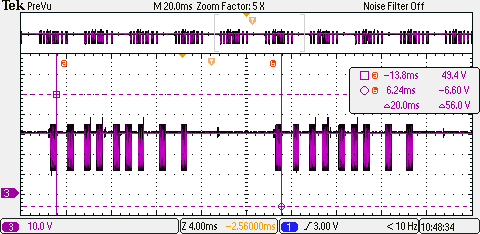
\includegraphics[width=0.6\textwidth]{fig_motor/Controller_Treiber/GraupnerGR16_8_Frame.png}
	\caption[8 Channel Frame]{8 Channel Frame}
\end{figure}

Es gibt zwei M�glichkeiten: ein Frame mit acht Kan�len, bestehend aus neun Peaks und acht Pausensignalen...

\begin{figure}[H]
	\centering
	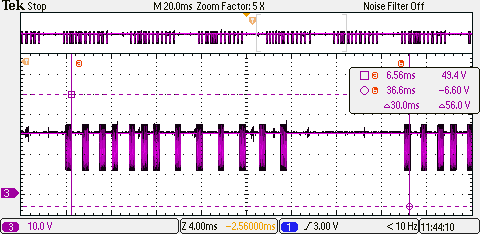
\includegraphics[width=0.6\textwidth]{fig_motor/Controller_Treiber/GraupnerGR16_12_Frame.png}
	\caption[12 Channel Frame]{12 Channel Frame}
\end{figure}

... oder einen 12 Kan�len Frame, bestehend aus 13 Peaks und 12 Pausensignalen.

\begin{figure}[H]
\centering
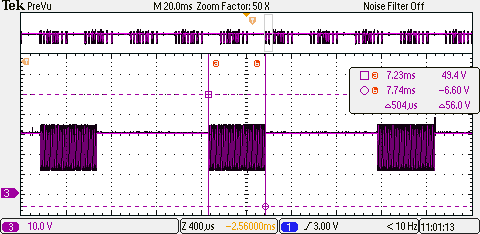
\includegraphics[width=0.6\textwidth]{fig_motor/Controller_Treiber/GraupnerGR16_8_ChX_Gap.png}
\caption[Dauer 8 chanel Frame ]{Dauer 8 Chanel Frame}
\end{figure}

Folgend die Anschaung eines Frames mit acht Kan�len mit der Dauer von 504us.

\begin{figure}[H]
	\centering
	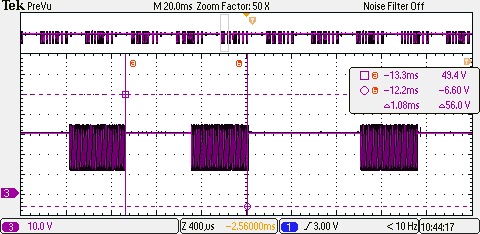
\includegraphics[width=0.6\textwidth]{fig_motor/Controller_Treiber/GraupnerGR16_8_Ch1_Min.png}
	\caption[Minimale Pause zwischen Frames]{Minimale Pause zwischen Frames}
\end{figure}

Zu sehen ist hier der kleinstm�gliche zeitliche Abstand zwischen zwei Frames mit der Dauer von nur 504us.

\begin{figure}[H]
	\centering
	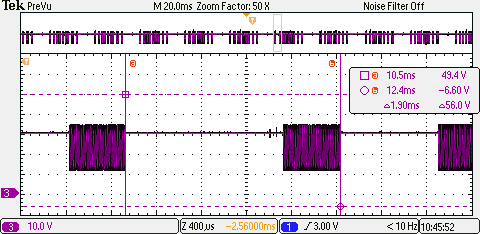
\includegraphics[width=0.6\textwidth]{fig_motor/Controller_Treiber/GraupnerGR16_8_Ch1_Max.png}
	\caption[Maximale Pause zwischen Frames]{Maximale Pause zwischen Frames}
\end{figure}

Hier ein Ausschnitt mit dem gr��tm�glichen Abstand zwischen zwei Frames mit der Dauer 1,396ms.

\section{Hardware Layout}
F�r die schnelle Durchf�hrung von �nderungen, Erweiterungen oder Anpassungen an der Hardware werden die Leiterplatinen und Schaltpl�ne mittels Tool elektronisch festgehalten. Die dazu m�gliche Software sind: EAGLE oder Fritzing,
die kostenlos oder als eingeschr�nkte Freeversion angeboten werden, aber diversen Einschr�nkungen unterliegen. Beide Tools haben eine Community, die viele Bauteile in Liberias bereitstellt. 

Im direktem Vergleich macht EAGLE einen professionelleren Eindruck und bietet eine Sammlung von Tutorials und Libraries. Aus diesen Gr�nden fiel die Entscheidung auf die EAGLE SOFTWARE. Es sollte aber mit dem Platz m�glichst sparend umgegangen werden, da bei dieser Freeeware die Gr��e und Anzahl der Layouts begrenzt ist.

\subsection{HElicopter Schematic Layout}

Es wurde f�r die schematischen Zeichnungen ein EAGLE Projekt angelegt, dass die schematischen Zeichnungen aller selbst gebauten bzw. zusammengef�gten Bauteile enth�lt. Das Projekt File ist im Verzeichnis \textit{trunk/hardware/} unter \textit{HElicopterPlus} abgespeichert.

Derzeit befinden sich zwei verschiedene schematischen Zeichnungen im Projektverzeichnis, die maximal aus zwei sogenannten Sheets besteht (Begrenzung durch die Freeware-Version von EAGLE). Der erster Sheet beinhaltet immer, denn Komplettaufbau des jeweiligen Systems. Der zweite Sheet wird verwendet um druckbare Versionen das Schaltplans zu erstellen (DINA4 Frame). Hierbei ist es wichtig, eine �bersichtliche Abspaltung vorzunehmen. 


\newpage
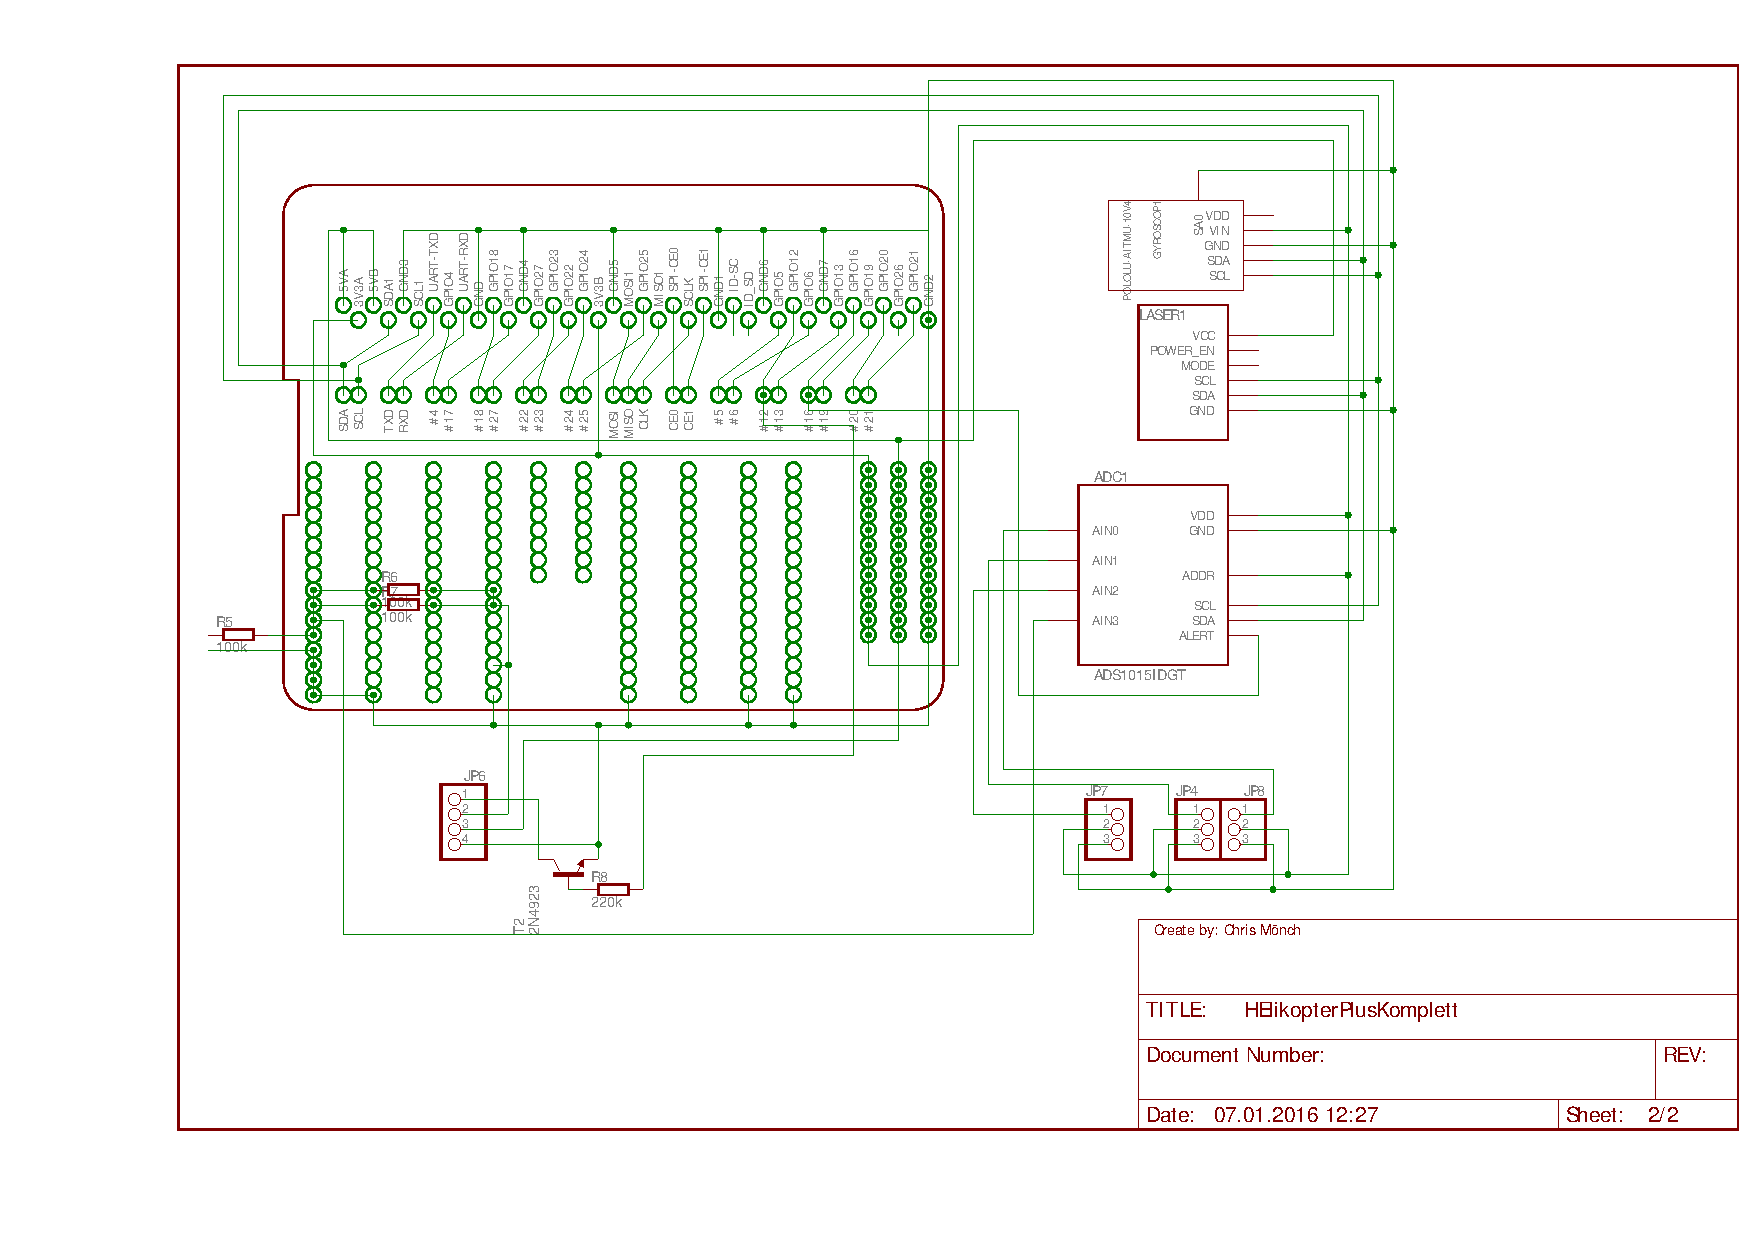
\includepdf[landscape=true,pages={1,2}]{fig_motor/Schematic/SchematicKomplettPrintVersion.pdf}
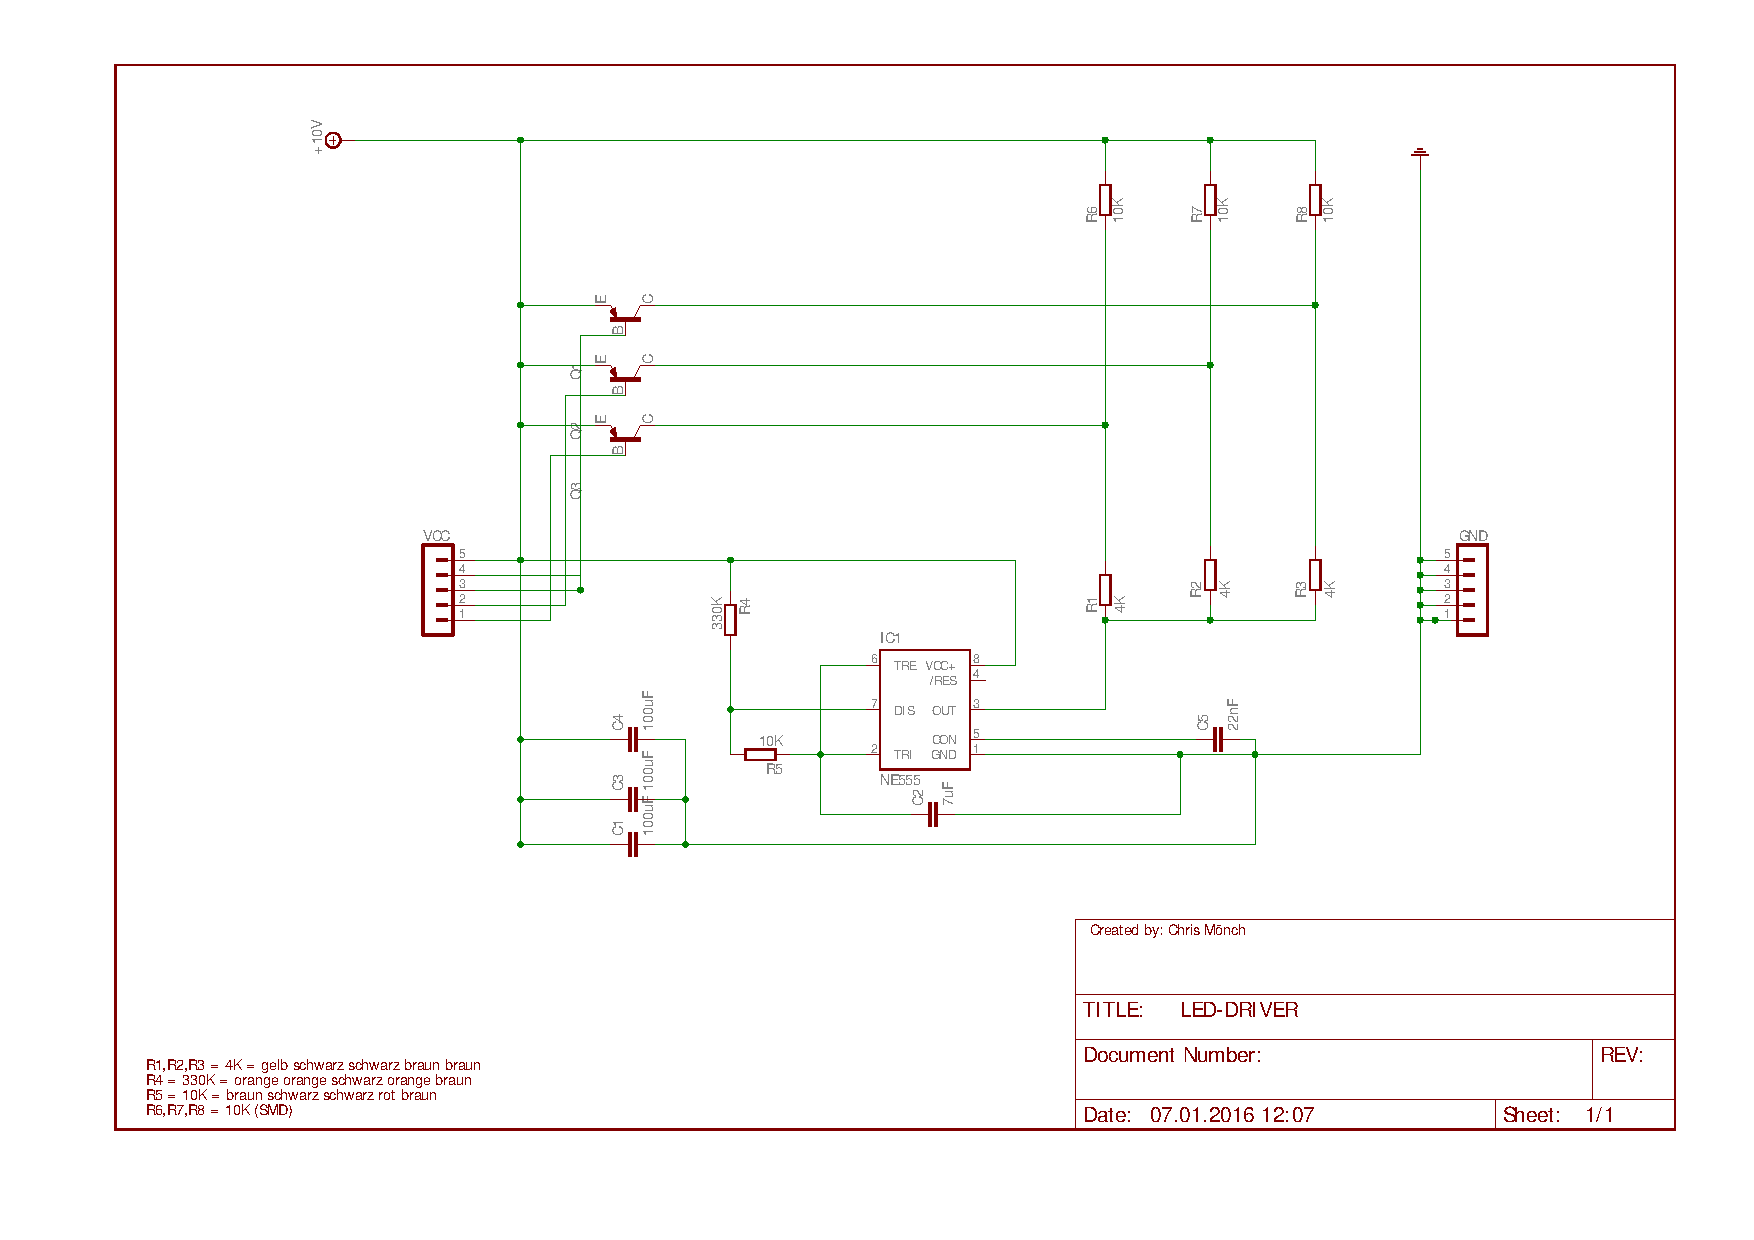
\includepdf[landscape=true]{fig_motor/Schematic/SchematicLedDriver.pdf}

\subsubsection{Richtlinien\cite{doc:guidelinesSchematics}}

\begin{itemize}
	\item Platzierung von mindestens einem Frame in jedem Sheet
	\item Verwendung von "Common" Symbolen
	\item Jedem Bauteil einen Wert zuordnen (wenn m�glich)
	\item F�r Verbindungen ausschlie�lich \textit{Net} verwenden ( nicht \textit{Wire})
	\item Verbindungen oder �berbr�ckungen wie in Abb. \ref{CrossingConnection} dargestellt
	\item Abk�rzungen direkt in dem jeweiligen Sheet festhalten
	\item Name und Bauteile immer in eine Richtung flie�en lassen (wenn m�glich)
	\item �berbr�cken von Netzen m�glichst gering halten
	\item F�r gro�e schematische Skizzen immer auch druckbare Versionen in DINA4 Format erstellen
	\item Wichtigen Netzen immer einen Namen zuordnen (GND, +5V, SDA, SLC, ...)
	\item Namen und Bezeichnungen kurz halten
\end{itemize}

\begin{figure}[H]
	\centering
	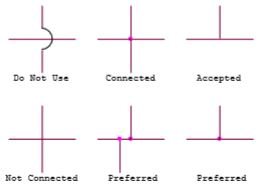
\includegraphics[width=0.5\textwidth]{fig_motor/Schematic/CrossingConnection.jpg}
	\caption[Net verbinden/�berbr�cken]{Net verbinden/�berbr�cken\protect\footnotemark}
	\label{CrossingConnection}
\end{figure}
\footnotetext{\url{http://www.k-state.edu/ksuedl/publications/Technote\%208\%20-\%20Guidelines\%20for\%20Drawing\%20Schematics.pdf}}


\newpage
\subsection{HElicopter Libary}
Auf der Bibliothek von Eagles k�nnen unter der Rubrik \emph{Downloads} Bauteile zu denn Schaltpl�nen gefunden werden. Die dort vorhandenen Bibliotheken sind von Usern bereitgestellt worden. Deshalb besteht die M�glichkeit, dass Bauteile fehlerhaft sind.

Wenn in der Bibliothek kein Element f�r das Bauteil gefunden werden konnte, muss dieses erstellt und in der bereits vorhandene Libary \textit{HElicopterLib.lbr} hinzugef�gt werden. In dieser Libary sind alle Teile festgehalten, die f�r die Quadrocopter ben�tigt werden. 

Ein Bauteil oder auch ein Device besteht aus insgesamt drei eigenen Bestandteilen, die alle vorhanden sein m�ssen, um das Bauteil zu verwenden:
\begin{center}
	\begin{tabular}{l p{10 cm} }
	Symbol & Darunter versteht man eine schematische Skizze eines Bauteils. Alle Schnittstellen des Bauteiles sind zu erkennen und ggf. zu kennzeichen. \newline Der Orignalma�stab und Echtheit der Pinanordnung spielt keine Rolle. Diese soll m�glichst so platziert werden, um im sp�teren Layout eine gewisse �bersichtlichkeit zu wahren. Die Namen der Pins sollen so benannt werden, wie diese vom Hersteller in den Datenbl�ttern festgelegt ist. Ansonsten k�nnte es Sp�ter Probleme zur Pin-Zuordnung geben \newline Die Schl�sselw�rter \textit{>NAME} und \textit{>VALUE} sollen sich (wenn m�glich) im Symbol befinden. \\
	Package & In dieser Skizze soll eine realit�tsnahe Abbildung des Bauteiles erstellt werden, mit original Abmessungen wie z.B. Platinengr��e, Platinenform, Pins und Bohrl�cher, die aus den jeweiligen Datenbl�ttern ersichtlich sind. 
	Weitere Erg�nzungen sind sonstige Bauteile oder SMD auf einem Device sowie deren Verbindungen auf Ober- bzw. Unterseite. Diese werden derzeit nicht ben�tigt und wurden deshalb weggelassen. \\
	Device & In einem Device werden ein Symbol und ein Package miteinander zusammengef�gt. Die Pins aus dem Symbol und Package Skizzen werden  miteinander verkn�pft. Wenn jeder Pin zugeordnet wurde kann das Device verwendet werden.\\
	\end{tabular}
\end{center}

Der Vorteil dieser Aufteilung ist der, dass einzelne Packages und Symbole f�r mehrere Devices verwendet werden k�nnen. Nur die Anzahl der Pins aus den Packages und Symbolen m�ssen eindeutig �bereinstimmen und zugewiesen werden.

\subparagraph{Um bereits existierende Libaries hinzuzuf�gen} wird die gew�nschte Libary in dem Ordner EAGLE-7.5.0/*lbrName* gespeichert. Anschlie�end klickt man im Reiter \emph{Bibliothek} auf \emph{Benutzen} und w�hlt die gew�nschte Libary aus. Ein Schaltplan muss hierbei ge�ffnet sein. Im \textit{Controll Panel} ist das Hinzuf�gen von libaries nicht m�glich. Zuletzt m�ssen die libaries noch aktualisiert werden( unter \emph{Bibliothek} auf die Rubrik \emph{Alle Aktualisieren}). Abschlie�end auf  \textit{ Add/Neues Bauteil hinzuf�gen}, es erscheint die Libary in der Liste. 

\subparagraph{Um ein vorhandenes Bauteil in die eigene Libary einzuf�gen} muss die Ziel-Libary ge�ffnet sein. Im \textit{Control Panel} von EAEGLE( in der linken Spalte das Men� \textit{Bibliotheken} �ffnen). Hier sollten sich alle bereits hinzugef�gten Libaries befinden. Ist dies nicht der Fall: rechtsklick auf die \textit{Bibliotheken} und  \textit{alle Bibliotheken laden} ausw�hlen. Nun muss die Quell-Libary des Bauteils ge�ffnet werden.Das zu kopierende Bauteil rechts klicken und \textit{In Bibliothek} ausw�hlen. Es ist auch m�glich, einzelne Packages oder Symbole neben ganzen Bauteilen/Devices zu kopieren. Nun sollte das hinzugef�gte Objekt in der Ziel-Libary ge�ffnet sein. Best�tigen sie das Hinzuf�gen mit Speichern der Libary.

\subparagraph{F�r das Bearbeiten existierender Libaries} �ffnen sie eine schematische Skizze. Klicken sie auf \textit{Bibliothek}, dann \textit{�ffnen..} und w�hlen sie die zu �berarbeitende Libary aus. Nun k�nnen alle existierende Bauteile, Packages und Symbole bearbeitet oder neue erstellt werden.
Nach der �nderung speichern Sie die Libary und klicken sie auf wieder auf Bibliothek. Anschlie�end aktualisieren Sie die Libaries. Die �nderungen sollten nun vorgenommen sein.

\textit{Achtung:} �nderungen werden auf alle bestehenden und eingef�gten Elementen vorgenommen. Dies kann sich z.B. unvorteilhaft auf die Lesbarkeit auswirken. Aus diesem Grund sollte zumindest eine Kopie des ge�nderten Devices oder eine neue Version erstellt werden. 


\chapter{Ausblick}

F�r die Flugf�higkeit des Quadrocopters sollten folgende Themen bearbeitet werden:

\paragraph{ Behebung des Fehlers der VMware } wurde im folgenden Abschnitt \ref{vmWareError}. \nameref{vmWareError} auf S.\pageref{vmWareError} beschrieben. Um f�r weitere Projektarbeiten wieder das Arbeiten mit der VMware zu erm�glichen sollte dieses Problem gel�st werden.

\paragraph{ Die verwendeten Scripts local} und nicht mehr �ber ssh Zugriff starten lassen und z.B. per UDP die Daten an das Raspberry �bertragen.

\paragraph{ Entwicklung von Stabilit�tsregelung} f�r vertikales und horizontales Halten.

\paragraph{ Anbindung der Fernsteuerung } mittels GR-16 (siehe Abschnitt \ref{Controller Treiber}. \nameref{Controller Treiber} auf S.\pageref{Controller Treiber} ) mit einem externen PPM-Decoder oder �ber den Echtzeitf�higen installierten Linux Kernel. 

% % %%%%%% Anhang
\appendix
\chapter{Code}
\label{sec:a-kapitel}


\label{motorH}
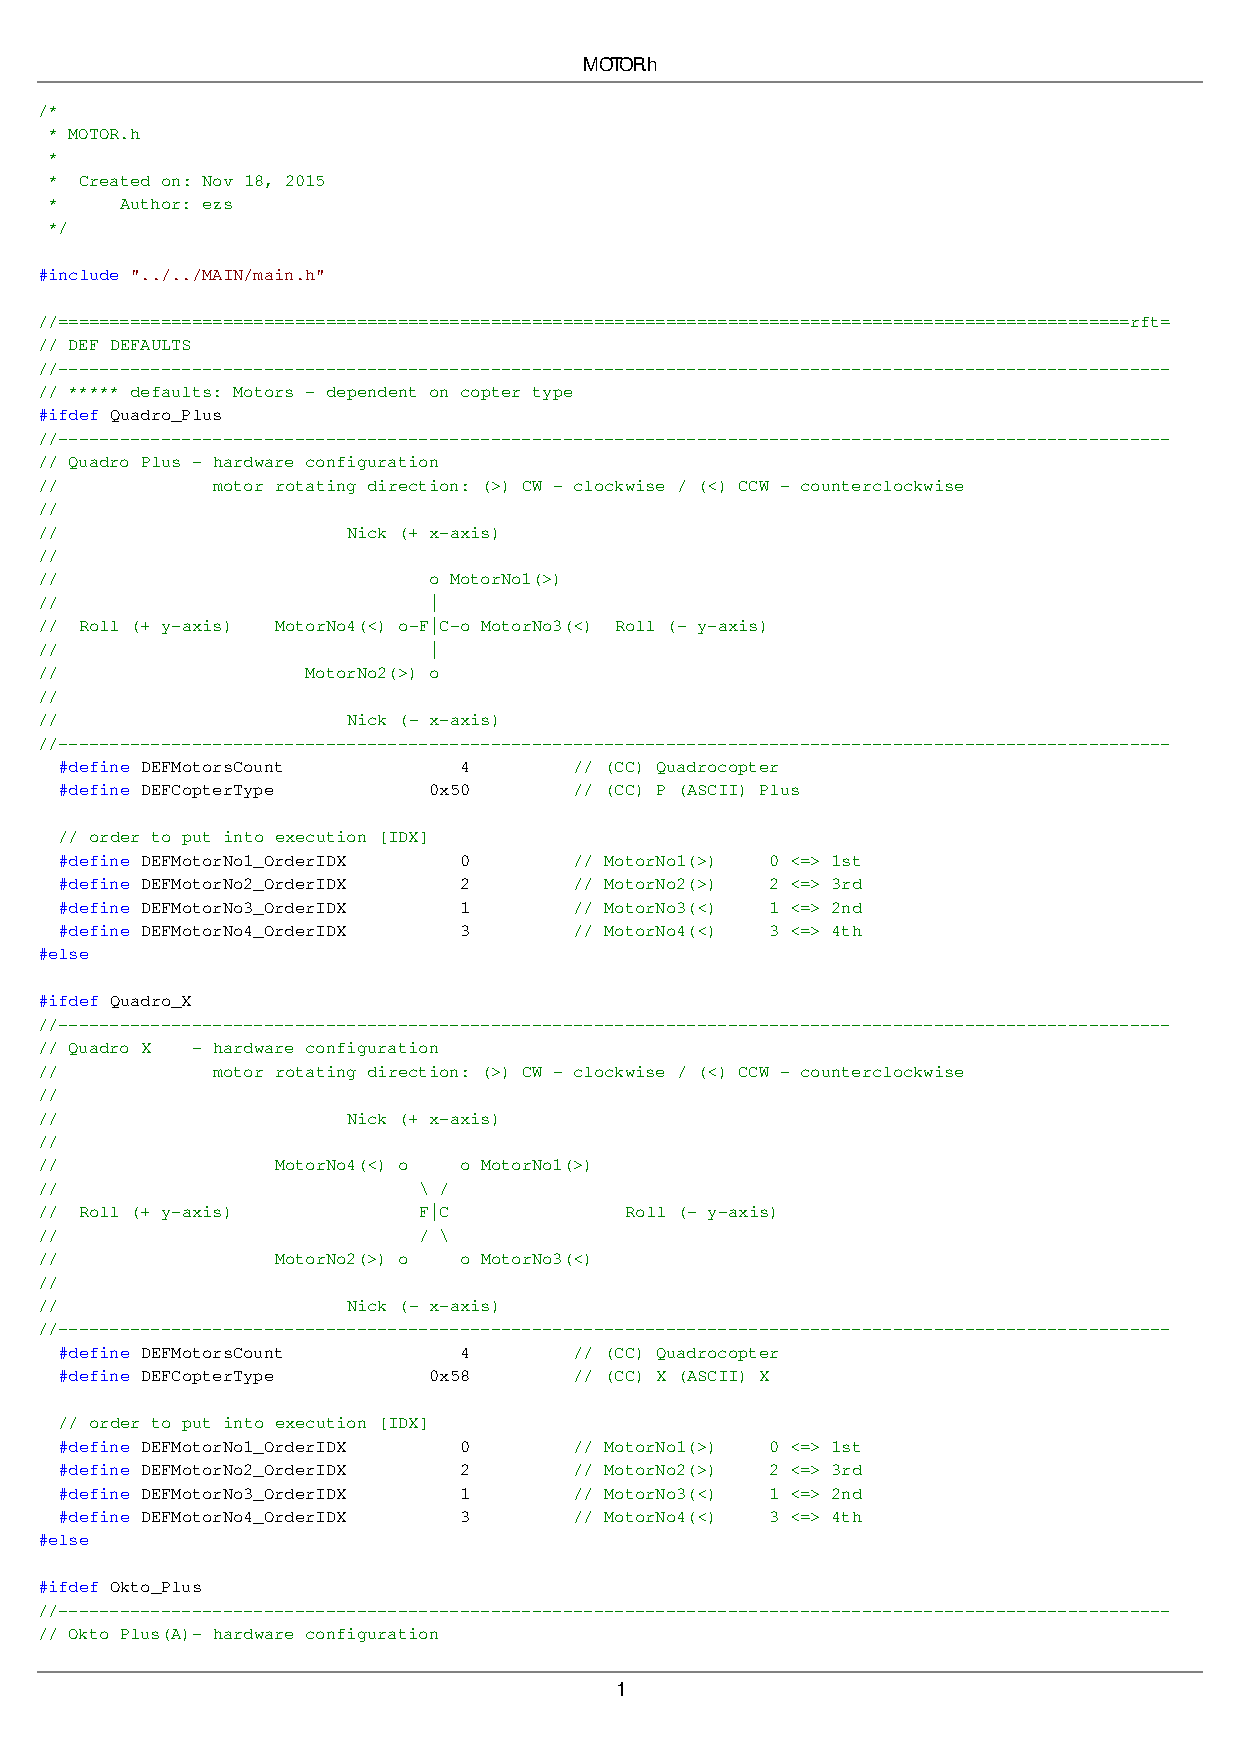
\includepdf[pages={1,2,3}]{fig/pdf/MotorH.pdf}

\section{Script \textit{'testcase'}}
\label{script_testcase}
\begin{lstlisting}[language=bash]
#!/bin/bash
#Sets or Clear Flag to Run a testcase
#Used Parameter:
#	$1 - Testcase name which to set or clear
#	$2 - Optional Parameter set or clear the Testcase,if Unknown testcase will be set

#Path of file where all testacses are stored:
path="/home/pi/testfiles/_Testcases" 

if [ "$1" == '' ]
then
echo "First Paremeter does not exist, expected name of a testcase"
exit 1
else 
testcase=$1
fi

if [ "$2" == "clear" -o "$2" == "set" ]
then
if [ "$2" == "clear" ] 
then
mode=0
else
mode=1
fi
echo "mode $2 is used" 
else
mode=1
echo "used default mode set"
fi

if [ -e $path ]
then
echo "$path found"
else
echo "$path not found"
exit 2
fi

sed -i "s/^$testcase=[01]/$testcase=$mode/" $path
if [ $? == 0 ]
then echo "Command executed"
fi
\end{lstlisting}


% % %%%%%% Literaturverzeichnis (darf im deutschen nicht in den Anhang!)
% Einfaches Literaturverzeichnis
\begin{thebibliography}{XXXX}
\bibitem{doc:gt-16} Graupner/SJ Gmbh, Bedienungsanleitung Graupner HoTT 2.4,  \url{http://www.graupner.de/mediaroot/files/33508_Kurzanleitung_de.pdf}; 
\textit{Januar 2011 DE V1.3}

\bibitem{doc:ppm} Herbert Bernstein, Informations- und Kommunikationselektronik, Walter de Gruyter GmbH, 2015,  \textit{1. Auflage}

\bibitem{doc:gpsHat} Lady ada/Adafruit Industries, Adafruit Ultmate GPS HAT for Raspberry Pi, \url{https://learn.adafruit.com/downloads/pdf/adafruit-ultimate-gps-hat-for-raspberry-pi.pdf},  \textit{2016-01-11}

\bibitem{doc:gpsADC} Bill Earl/Adafruit Industries, Adafruit 4-Channel ADC Breakouts, \url{https://learn.adafruit.com/downloads/pdf/adafruit-4-channel-adc-breakouts.pdf},  \textit{2014-11-30}

\bibitem{doc:imu} Pololu Robotics \& Electronics, AAltIMU-10 v4 Gyro, Accelerometer, Compass, and Altimeter (L3GD20H, LSM303D, and LPS25H Carrier), \url{https://www.pololu.com/product/2470},  \textit{2016-01-13}

\bibitem{doc:lidar}EXP Tech, LIDAR-Lite v2, \url{http://www.exp-tech.de/lidar-lite-v2},  \textit{2016-01-13}

\bibitem{doc:guidelinesSchematics}Olin Lathrop, Rules and guidelines for drawing good schematics, \url{http://electronics.stackexchange.com/posts/28255/revisions},  \textit{2016-01-14}


\bibitem[Gun04]{doc:gun} Karsten G�nther, LaTeX2 --- Das umfassende Handbuch, Galileo Computing, 2004, \url{http://www.galileocomputing.de/katalog/buecher/titel/gp/titelID-768}; \textit{1. Auflage}
\end{thebibliography}



% Literaturverzeichnis mit Bibtex
%\bibliography{bib/bib}

% %  Inhalt ENDE %%%%%%%%%%%%%%%%%%%%%%%%%%%%%%%%%%%%%%%%%%%%%%%%%%%%%%%%%%
\end{document}
